\documentclass[a4paper,11pt]{article}

% CJK support: prefer ctex, fallback to XeTeX native line breaking
\IfFileExists{ctex.sty}{
  \usepackage[fontset=fandol]{ctex}
}{
  \usepackage{fontspec}
  \XeTeXlinebreaklocale "zh"
  \XeTeXlinebreakskip = 0pt plus 1pt
  \IfFontExistsTF{Noto Serif CJK SC}{\setmainfont{Noto Serif CJK SC}}{}
  \IfFontExistsTF{Noto Sans CJK SC}{\setsansfont{Noto Sans CJK SC}}{}
}

\renewcommand{\contentsname}{目录}
\renewcommand{\figurename}{图}
\renewcommand{\tablename}{表}

% ===== Colors =====
\usepackage{xcolor}
\definecolor{accent}{RGB}{60,113,183}
\definecolor{important}{RGB}{46,125,50}
\definecolor{warning}{RGB}{198,40,40}

\usepackage{amsmath, amssymb}
\usepackage{graphicx}
\usepackage[a4paper, top=3.0cm, bottom=2.8cm, left=2.6cm, right=2.6cm, headheight=15pt]{geometry}
\usepackage[most]{tcolorbox}
\usepackage{etoolbox}
\usepackage{listings}
\usepackage{booktabs}
\usepackage{subcaption}
\usepackage{float}
\usepackage{tikz}
\usetikzlibrary{positioning, shapes.geometric, calc}

% allow generous stretching to avoid overfull hboxes in CJK paragraphs
\emergencystretch=4em

% ===== Book layout =====
\usepackage{fancyhdr}
\pagestyle{fancy}
\fancyhf{}
\fancyhead[L]{\small\sffamily\nouppercase{\notetitle}}
\fancyhead[R]{\small\sffamily\nouppercase{\rightmark}}
\fancyfoot[C]{\small\thepage}
\renewcommand{\headrulewidth}{0.4pt}
\renewcommand{\headrule}{{\color{accent!45}\hrule width\headwidth height\headrulewidth}\vspace{-\headrulewidth}}
\fancypagestyle{plain}{%
  \fancyhf{}%
  \fancyfoot[C]{\small\thepage}%
  \renewcommand{\headrulewidth}{0pt}%
}

\usepackage{titlesec}
\titleformat{\section}[hang]
  {\Large\sffamily\bfseries\filright}
  {\textcolor{accent}{\Large\thesection}}
  {0.6em}
  {}
\titlespacing*{\section}{0pt}{1.6\baselineskip}{0.9\baselineskip}
\titleformat{\subsection}[hang]
  {\large\sffamily\bfseries}
  {\textcolor{accent}{\thesubsection}}
  {0.7em}
  {}
\titlespacing*{\subsection}{0pt}{1.1\baselineskip}{0.5\baselineskip}
\titleformat{\subsubsection}[hang]
  {\normalsize\sffamily\bfseries}
  {\textcolor{accent}{\thesubsubsection}}
  {0.7em}
  {}
\titlespacing*{\subsubsection}{0pt}{0.9\baselineskip}{0.4\baselineskip}

\usepackage{tocloft}
\renewcommand{\cftsecfont}{\sffamily\bfseries}
\renewcommand{\cftsecpagefont}{\sffamily\bfseries}
\renewcommand{\cftsubsecfont}{\sffamily}
\renewcommand{\cftsubsecpagefont}{\sffamily}
\renewcommand{\cftsubsubsecfont}{\sffamily}
\setlength{\cftbeforesecskip}{4pt}
\setlength{\cftbeforesubsecskip}{2pt}

% ===== Highlight boxes =====
\tcbset{
  ltnbox/.style={
    enhanced, breakable, sharp corners, boxrule=0.6pt,
    left=12pt, right=12pt, top=9pt, bottom=9pt
  }
}
\newtcolorbox{knowledgebox}[1]{
    ltnbox, colback=accent!4!white, colframe=accent,
    before upper={\textbf{\color{accent}#1}\par\smallskip}
}
\newtcolorbox{importantbox}[1]{
    ltnbox, colback=important!5!white, colframe=important,
    before upper={\textbf{\color{important}#1}\par\smallskip}
}
\newtcolorbox{warningbox}[1]{
    ltnbox, colback=warning!5!white, colframe=warning,
    before upper={\textbf{\color{warning}#1}\par\smallskip}
}

% ===== Transcript appendix formatting =====
% Used by transcript_appendix.tex (generated from the cleaned subtitle track)
\newcommand{\transcriptsec}[1]{\par\addvspace{0.9em}\noindent{\sffamily\bfseries\color{accent}#1}\par\addvspace{0.15em}}
\newcommand{\transcriptitem}[2]{\par\noindent\textbf{\footnotesize\sffamily\color{accent!80!black}#1}~#2\par\smallskip}

% ===== Figure provenance =====
\newcommand{\vtag}{\protect\footnotemark}
\newcommand{\srcnote}[1]{\footnotetext{视频画面时间区间：#1。若为裁剪图，时间区间仍对应原视频画面。}}

% ===== Front-page metadata =====
\newcommand{\notetitle}{Agentic 时代的漏洞研究}
\newcommand{\notesubtitle}{Black Hat USA 2026 主题演讲笔记：Yan Shoshitaishvili}
\newcommand{\notedate}{\today}
\newcommand{\videochannel}{Black Hat}
\newcommand{\videopublishdate}{2026--08--06}
\newcommand{\videoduration}{44 分 46 秒}
\newcommand{\videourl}{https://www.youtube.com/watch?v=VNYe3Cnk5Pw}
\newcommand{\videocoverpath}{cover.jpg}

% ===== PDF metadata and links =====
\usepackage[
  colorlinks=true,
  linkcolor=accent!85!black,
  urlcolor=accent!80!black,
  citecolor=accent!85!black,
  bookmarksnumbered,
  unicode
]{hyperref}
\hypersetup{pdftitle={\notetitle}, pdfsubject={\notesubtitle}}

\linespread{1.08}

\begin{document}

\pagenumbering{roman}
\pagestyle{fancy}
\setcounter{page}{1}

\begin{titlepage}
\thispagestyle{empty}
\setcounter{page}{1}
\centering
\vspace*{1.8cm}
{\Huge\sffamily\bfseries \notetitle\par}
\vspace{0.55cm}
{\Large\color{black!55} \notesubtitle\par}
\vspace{0.9cm}
{\color{accent}\rule{0.42\textwidth}{1.2pt}\par}
\vspace{1.2cm}

\includegraphics[width=0.72\textwidth,height=0.36\textheight,keepaspectratio]{\videocoverpath}\par

\vfill

\begin{tcolorbox}[
  enhanced, sharp corners, boxrule=0pt, toprule=0.5pt, bottomrule=0.5pt,
  colback=white, colframe=black!30,
  width=0.86\textwidth, left=10pt, right=10pt, top=9pt, bottom=9pt
]
\centering\small
\textbf{视频作者/频道}：\videochannel\par
\vspace{1pt}
\textbf{发布日期}：\videopublishdate \quad \textbf{视频时长}：\videoduration\par
\vspace{1pt}
\textbf{视频链接}：
\href{\videourl}{\nolinkurl{\videourl}}
\end{tcolorbox}

\vspace{0.7cm}
{\small\color{black!55} \notedate\par}
\vspace*{1.2cm}
\end{titlepage}

\clearpage
\tableofcontents
\thispagestyle{plain}

\clearpage
\pagenumbering{arabic}
\thispagestyle{plain}

%% --- 正文内容开始 --- %%

\section{开场：一场关于「人的位置」的主题演讲}

2026 年 8 月 6 日，Black Hat USA 2026 的最后一天，亚利桑那州立大学（ASU）副教授 Yan Shoshitaishvili 走上主舞台，发表主题演讲《Vulnerability Research in the Agentic Age（Agentic 时代的漏洞研究）》。他对自己的定位是：以漏洞分析、利用与修复为优先研究方向的学术研究者，同时是 CTF 社区的老牌选手——二进制分析框架 angr 的作者、CTF 战队 Shellphish 的核心成员、DEF CON CTF 组织者 Order of the Overflow 的成员。这场演讲因此天然带着双重身份：它既是前沿研究成果的发布，也是一个从攻击竞赛里长大的研究者对整个行业的自省。

视频以一段新闻蒙太奇开场：画外音反复播报「大规模网络攻击」「这可能是有史以来最大的一次」「美国正遭受虚拟入侵」。这是大会制作的片头，用危机感把观众带进议题；本讲义把它当作氛围铺垫，而不是论据来源。真正提出问题的是 Black Hat 总裁 Suzie Pallett 的开幕致辞：AI 正在从根本上改变「我们如何发现漏洞、威胁以多快的速度移动、我们如何分析它们」。她把整场 keynote 的命题压缩成一句话——当机器寻找缺陷的速度超过人类之后，人的位置在哪里？

Shoshitaishvili 给出的答案不是「人被取代」，而是「人被放大」。要理解这句话，需要先看清他身后的社区脉络。

\subsection{演讲者与 CTF 社区的方法论起点}

Black Hat 创始人、DEF CON 主席 Jeff Moss 在介绍演讲者时花了一半篇幅讲历史。大约 30 年前，夺旗赛（Capture the Flag，CTF）在 DEF CON 的一场网络对战中「意外诞生」。它起初不是教学工具，而是纯粹的攻防对抗；唯一被写进规则的典故来自第一年——参赛者攻陷了计分系统和路由器，于是第二年规定不准再打这些目标。这段历史被 Moss 提炼成一句话：\textbf{攻击为防御提供地面真相}（attack informs defense）。不了解攻击者实际如何构造漏洞利用，就做不出有效的防御。

Shoshitaishvili 的个人经历恰好是这条原则的产物。他母亲在俄罗斯取得了计算机科学博士学位；柏林墙倒塌后，俄罗斯学界被要求为政治候选人背书，当 KGB 上门施压时，8 岁的他随家人逃往美国。大学里他迷上 CTF 并把大量手工逆向工作自动化——这最终变成了 angr，一个结合静态与动态符号执行的二进制分析平台。凭借它，Shellphish 在约两年的全球竞赛中几乎「通吃」。angr 此后被超过 1000 个研究、学术与产品工具采用（讲者自述数字），战队又顺势组建 Order of the Overflow 接手 DEF CON CTF 的组织工作。Moss 用一句话总结这条轨迹：漏洞利用的开发正在\textbf{从手艺变成科学}。

\subsection{本章小结}

这场 keynote 的真正主角不是某个模型或某个工具，而是一个反转：当机器接管了「找漏洞」的体力活，漏洞研究反而更需要人的判断力。这个反转贯穿本讲义的后面七个章节，也决定了本讲义的结构。

\section{在 agent 之前：漏洞发现的三条规模化路径}

Shoshitaishvili 先调侃了自己的工作模式：学术研究者的典型流程是「在洗澡时产生灵感，把它交给聪明的 graduate student，他们把灵感实现成论文和原型」。agentic 时代把这个流程改成了「学生向 agent 提出需求，学生完成 agentic 原型，学生拿到结果」——研究者被推到离最终成果更远的位置。这个看似轻松的开场，其实是整场演讲的布局：工具在下沉，人在上移。

\subsection{Agentic 时代 $\neq$ LLM 时代}

演讲先划清一条边界：把代码全部粘贴进 ChatGPT 并不能「解决漏洞问题」。他引述了 keynote 前一天的新闻——苹果正在收紧其漏洞奖励计划，因为报告被 AI 幻觉产生的「slop（低质量垃圾报告）」淹没；这些报告来自不知道如何过滤幻觉的提交者\footnote{据 Financial Times 报道（MacRumors、Decrypt 等 2026 年 8 月初转载）：苹果自 2026 年 6 月起限制每位研究者同时打开的报告数并附加 30 天冷静期；米兰创业公司 Bynario 用 ChatGPT 三周发现 50 余个 macOS 潜在漏洞，其中一个提权链因配额耗尽无法提交。参见文末参考资料。}。讲者的态度是：这种混乱会被消化掉——模糊测试发展的每个阶段都经历过类似的阵痛。他不谈幻觉，只谈「最终会做事的人如何使用这些技术」。

\subsection{三种把漏洞发现自动化的方式}

讲者把所有「某方法发现 N 个漏洞」的研究与新闻归结为三条路径，并用一张幻灯片同时点出前两条（图~\ref{fig:three-ways}）。

\begin{figure}[H]
\centering
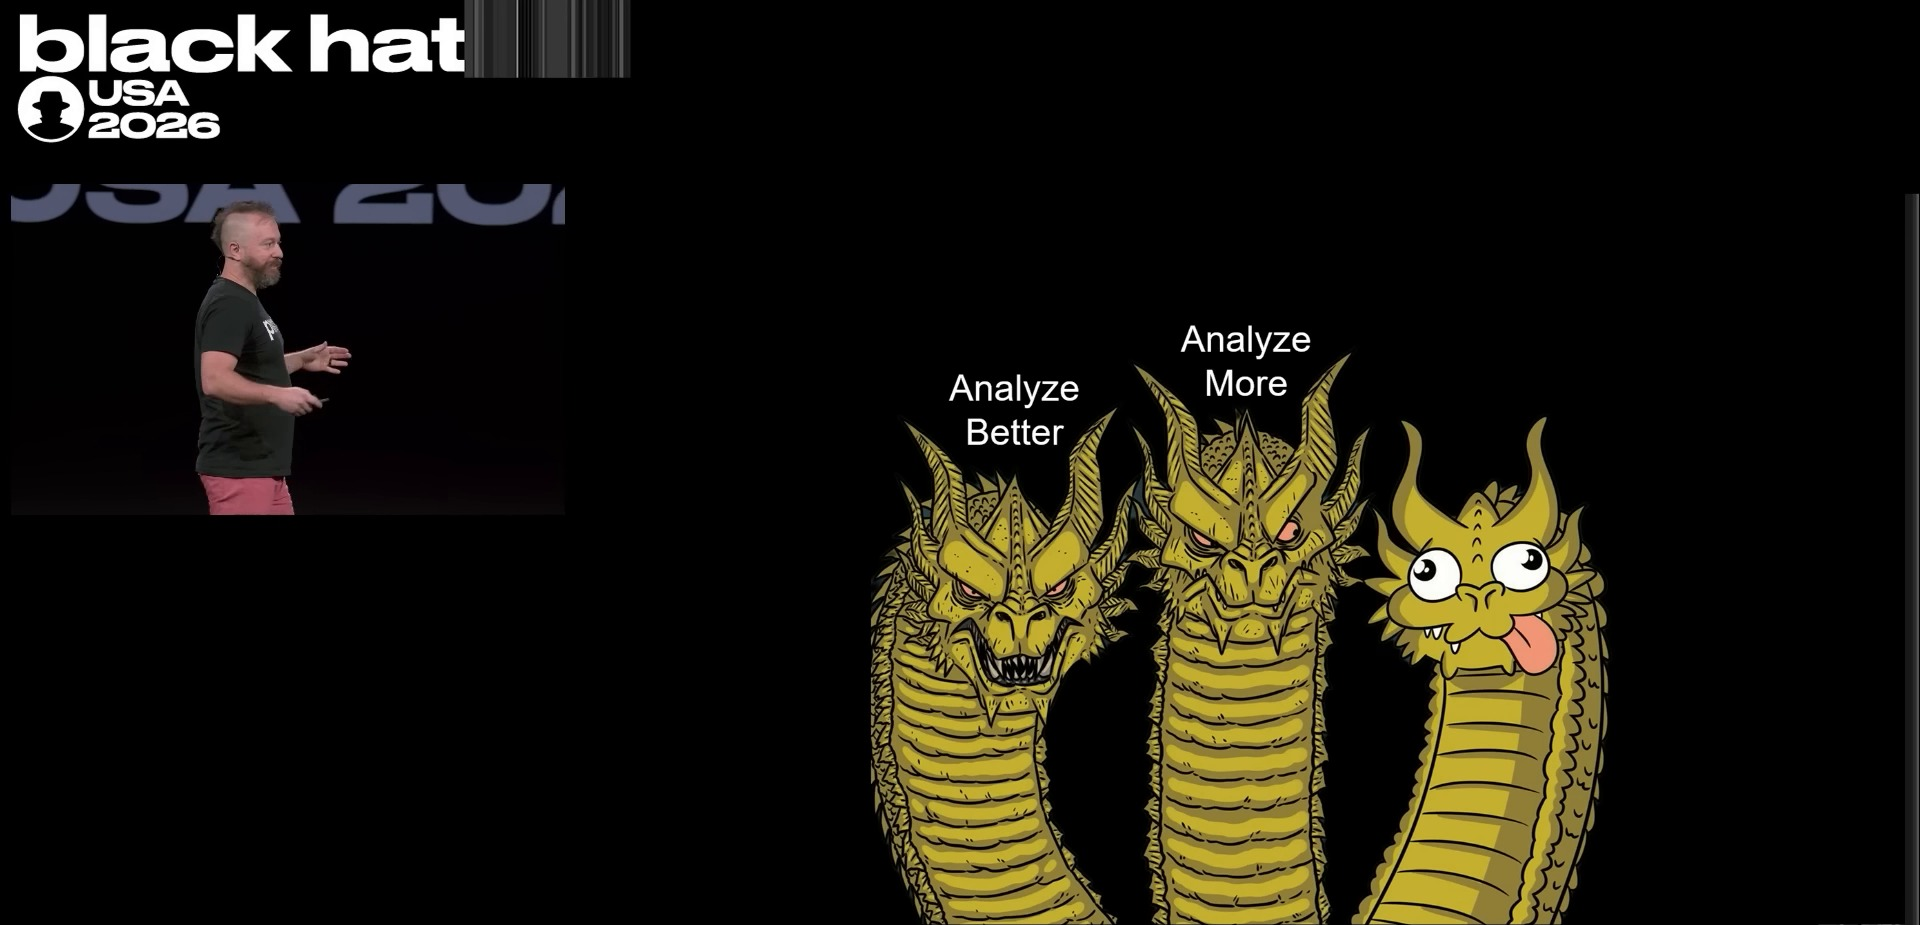
\includegraphics[width=\textwidth]{figures/fig_01_three_ways.jpg}
\caption{「更好地分析」与「分析更多」两条路径的幻灯片（画面底部 Black Hat 字样已裁掉）\vtag}
\label{fig:three-ways}
\end{figure}
\srcnote{00:15:14--00:15:29}

第一条是\textbf{更好地分析}（Analyze Better）：把既有分析器做得更准、更快——更少误报、在超时之前跑完。他举的 agentic 例子是更强的模型能发现上一代模型漏掉的漏洞（后文的 Mythos 即属此类）。第二条是\textbf{分析更多}（Analyze More）：分析器不变，只扩大适用面——以前能分析 8 个程序，现在分析 800 个，漏洞数随之线性增长。第三条是\textbf{换个方式分析}（Analyze Differently）：甚至不需要更好的分析器，只要改变分析的视角，就能找到全新的漏洞。

第二条路径的注脚是 ARBITER：Shoshitaishvili 的学生 Jay Vadayath 在 angr 之上构建的分析平台，把二进制漏洞检测做到了仓库级规模——直接扫描 Linux 发行版软件仓库中的每一个程序。图~\ref{fig:arbiter} 是演讲展示的统计表。

\begin{figure}[H]
\centering
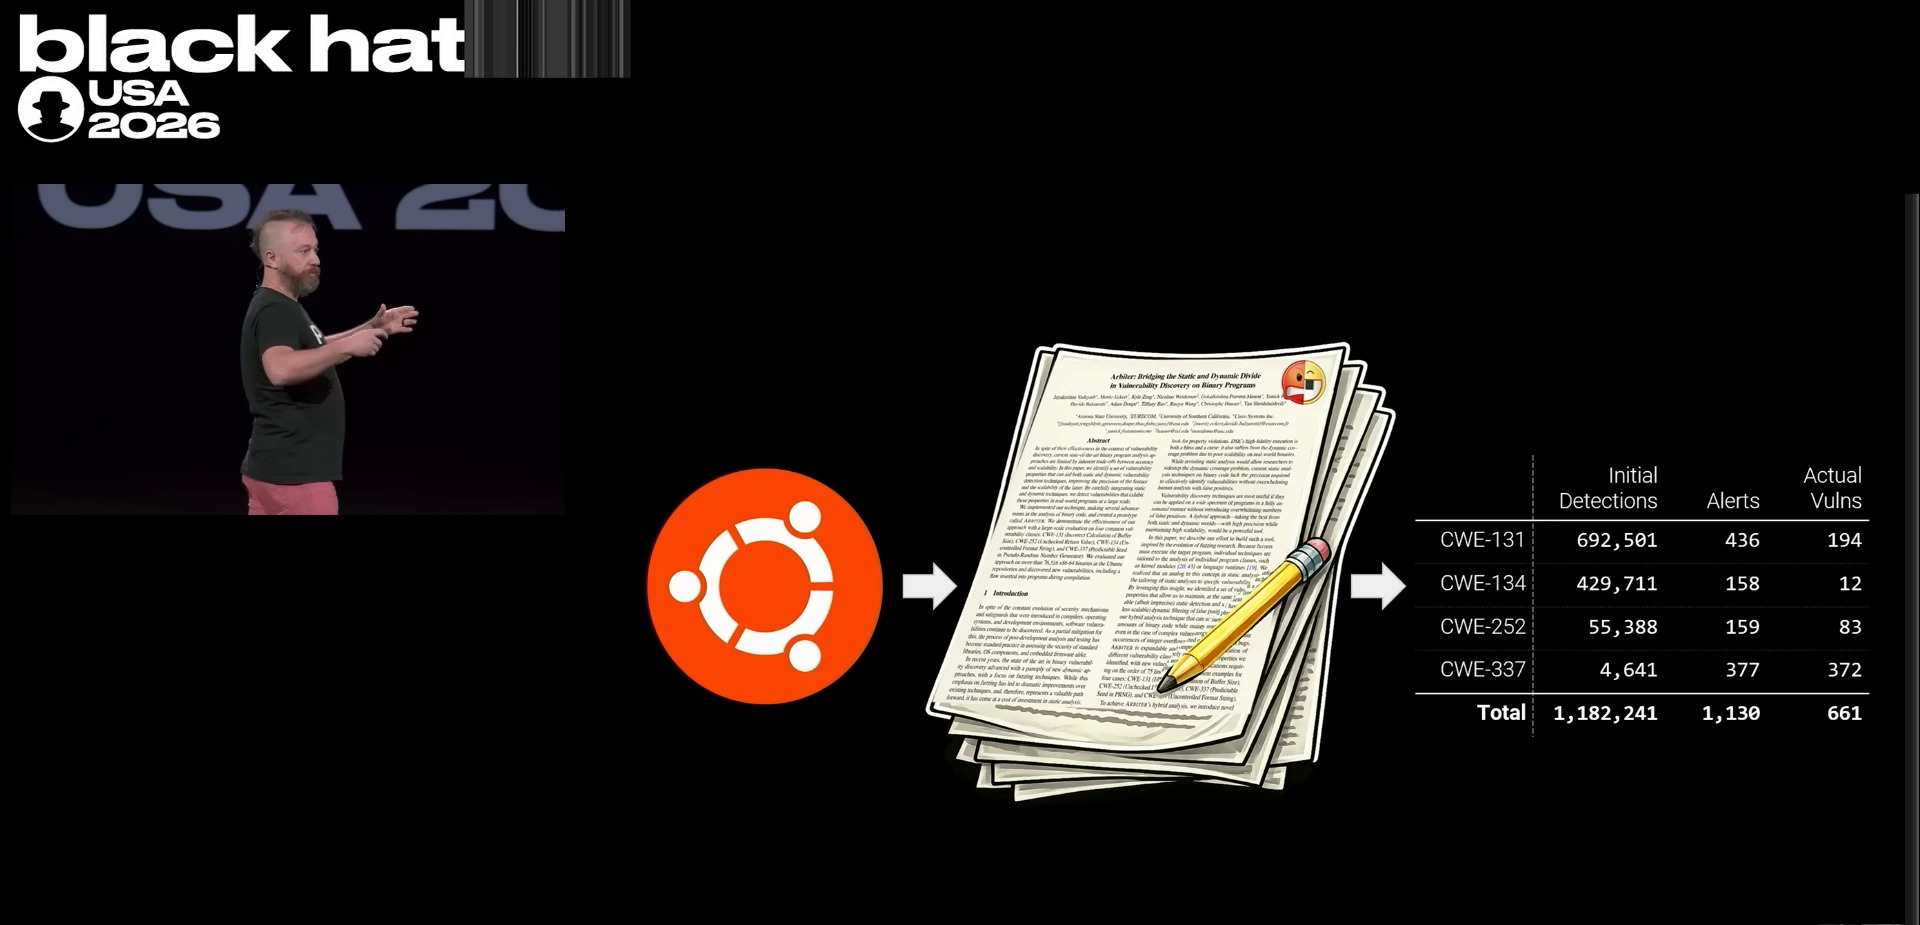
\includegraphics[width=\textwidth]{figures/fig_02_arbiter_table.jpg}
\caption{ARBITER 对仓库级二进制的扫描结果表：四类 CWE 合计 1,182,241 个目标、1,130 条报警、661 个漏洞（幻灯片 OCR 读数）\vtag}
\label{fig:arbiter}
\end{figure}
\srcnote{00:15:29--00:16:14}

作为参照，论文本身给出的样本规模是：ARBITER（USENIX Security 2022）在 76,516 个来自 Ubuntu 18.04 仓库的 x86-64 二进制上完成了评测\footnote{论文：\href{https://www.usenix.org/system/files/usenixsecurity22-vadayath.pdf}{Arbiter: Bridging the Static and Dynamic Divide in Vulnerability Discovery}。幻灯片上的计数口径与论文样本口径不同，二者并列于此，不强行调和。}。规模本身就是第二种路径的产出方式：工具没变强，靶子变多了。

\subsection{饼干模子：为什么「换个方式」能找到新漏洞}

第三条路径的解释依赖全场最核心的类比。把一个程序的全部漏洞想成一整块擀平的面团，每一种分析器都是一块饼干模子：静态分析按它的形状从面团上「扣出」一类漏洞，扣完之后再用同一块模子扣，扣不出新东西——不是代码变完美了，而是这种技术能看到的漏洞已经见底。换一块形状略有不同的模子（研究原型 B），只会扣出一小片新的边角料。

模糊测试（fuzzer，如 AFL）则是一块会随机晃动的模子：由于输入是随机生成的，即使重复压同一块面团，也会在边角处扣出前一次没扣到的形状。由此引出一个方法论后果：\textbf{重跑一次还有新产出，是随机性分析器的特性，而不是它更强的证据}。图~\ref{fig:cookie} 是本讲义根据这个类比绘制的示意图。

\begin{figure}[H]
\centering
\begin{tikzpicture}[scale=0.95]
  % dough
  \draw[fill=black!4, thick] plot[smooth cycle] coordinates
    {(-5.2,-1.6) (-4.4,-2.1) (-2.2,-2.2) (0,-2.3) (2.6,-2.0) (4.6,-1.4)
    (5.0,-0.2) (4.4,1.1) (2.4,1.9) (-0.2,2.1) (-2.9,1.8) (-4.7,0.9) (-5.4,-0.4)};
  \node[font=\sffamily] at (0,-2.7) {某程序的全部漏洞（未知边界）};
  % cutter shapes
  \draw[fill=accent!25, very thick, accent] (-4.3,0.2) circle (1.0);
  \node[font=\sffamily\small] at (-4.3,-1.3) {静态分析 A};
  \draw[fill=important!25, very thick, important] (-0.7,0.9) ellipse (1.3 and 0.7);
  \draw[fill=important!25, very thick, important] (0.5,0.4) ellipse (0.9 and 1.1);
  \node[font=\sffamily\small] at (0.0,-1.3) {静态分析 B（形状略不同）};
  \draw[fill=warning!25, very thick, warning] (3.5,-0.1) plot[smooth cycle] coordinates
    {(2.7,0.4) (3.2,1.0) (4.2,0.9) (4.6,0.1) (4.1,-0.7) (3.2,-0.6)};
  \draw[fill=warning!25, very thick, warning] (2.9,0.2) circle (0.35);
  \draw[fill=warning!25, very thick, warning] (4.1,0.5) circle (0.3);
  \node[font=\sffamily\small] at (3.6,-1.3) {模糊测试（随机形状）};
\end{tikzpicture}
\caption{「饼干模子」示意图（本讲义据讲者类比绘制，非视频画面）：每种分析器只扣出与其「形状」对应的漏洞子集；形状由它所针对的漏洞属性决定}
\label{fig:cookie}
\end{figure}

\subsection{工具之间其实很难比较}

最后一块拼图是评测困境。从 2013--2015 年前后 DARPA 网络大挑战（Cyber Grand Challenge）立项推动「自主漏洞研究」以来，行业经历了十年的「模糊测试复兴」：每年都有新 fuzzer 声称「我们换了个方式，在已经被 fuzz 过的代码里找到了新 bug，所以我们更强」。这类比较几乎无法成立——要公平比较两种分析器，必须把时间倒回原点、从零开始分别分析，而谁都做不到。LLM 让情况更糟：模型训练数据里混着历史上所有已知漏洞，它「发现」的到底是推理结果还是记忆污染，极难分辨。讲者的实验室正在做这件事，并已得到方向性结论：每种分析扣出的不是随机形状，而是由漏洞属性决定的形状。

\begin{knowledgebox}{漏洞属性为什么重要：本节的概念桥}
「饼干模子」的形状不是随便长的。它对应漏洞本身的性质——数据流走向、是否注入攻击者可控内容、是否依赖多线程行为等。分析器要么显式地选定这些性质（多数静态分析），要么隐式地被这些性质约束（直接把代码丢给 LLM、许多模糊测试）。承认这一点，是从「比谁的数字大」转向「比谁看得清」的转折点，也是下一节的全部主题。
\end{knowledgebox}

\subsection{本章小结}

三类路径——更准、更广、换视角——对应漏洞供给的三种扩张方式；而饼干模子类比说明：决定一个分析器能找到什么漏洞的，是它所针对的漏洞属性，而不是它的品牌或算力。至于「谁更强」的比较，在无法倒回时间的前提下，大多是顺序效应。这个结论把问题推向了下一节：与其追求更强的模子，不如先把「形状」本身研究清楚。

\section{漏洞属性：把第一个 0day 变成方法论}

\begin{importantbox}{漏洞属性（vulnerability properties）的定义}
一个漏洞可被利用，往往因为它满足若干可分离的性质：数据跨越了不可信边界、攻击者可控内容被注入到解释器、触发条件依赖多线程时序、逻辑漏洞绕过了身份认证等。这些性质不是漏洞的「标签」，而是漏洞的\textbf{成因结构}。分析器——无论静态、动态还是 LLM——实际针对的都是这些性质的子集。
\end{importantbox}

讲者的核心论点（thesis）就建立在这个定义上：进入 agentic 时代之后，竞争的关键不是模型参数量，而是\textbf{能否系统性地产出、表达和复用漏洞属性}。图~\ref{fig:thesis} 是他在幻灯片上写下的同一句论点。

\begin{figure}[H]
\centering

\includegraphics[width=\textwidth]{figures/fig_03_vuln_properties.jpg}
\caption{核心论点幻灯片「VULNERABILITY PROPERTIES IN THE AGENTIC AGE」\vtag}
\label{fig:thesis}
\end{figure}
\srcnote{00:22:29--00:22:59}

\subsection{案例：用 Android 的已知属性审计 OpenHarmony}

论点的第一个证据来自一篇在 keynote 之后一周正式发表的论文（USENIX Security 2026），第一作者是其学生 Hongkai Chen。研究对象是华为的 OpenHarmony：一个从零重新实现、参考 Android 设计的新操作系统，运行在 10 亿台设备上，但在 keynote 之前没有重量级的学术安全研究。

方法的链条很清晰：先系统梳理过去十余年 Android 安全研究中积累的漏洞，把这些漏洞\textbf{抽象成属性}（论文系统综述了 116 篇研究，提取出 56 个 Android 设计级漏洞，其中 24 个在 OpenHarmony 上被验证可复现\footnote{论文：\href{https://www.usenix.org/conference/usenixsecurity26/presentation/chen-hongkai}{SoK: History Doesn't Repeat Itself, but Android Design-Level Vulnerabilities Rhyme in OpenHarmony}。其中 Android 研究的挖掘环节由 agent 辅助完成。}），得到一本「属性配方书」；再带着这本配方书手工审计 OpenHarmony 的上百万行代码；每个被搬过去的属性，几乎都能在 OpenHarmony 里扣出一个新的 0day——最终找到数十个缺陷，从蓝牙设备接管到定位、通讯录等隐私泄露。

这个结果有两层意义。第一层是工程价值：属性可以\textbf{跨系统迁移}，新操作系统不再享受「没人研究我」的蜜月期。第二层是方法论价值：漏洞属性是可复制的知识资产，而 agent 的加入（先用 agent 辅助挖掘，再辅助应用）让「复制」本身也开始自动化。图~\ref{fig:sok} 与图~\ref{fig:dlv} 分别是论文题名页和演讲中展示的属性清单表。

\begin{figure}[H]
\centering
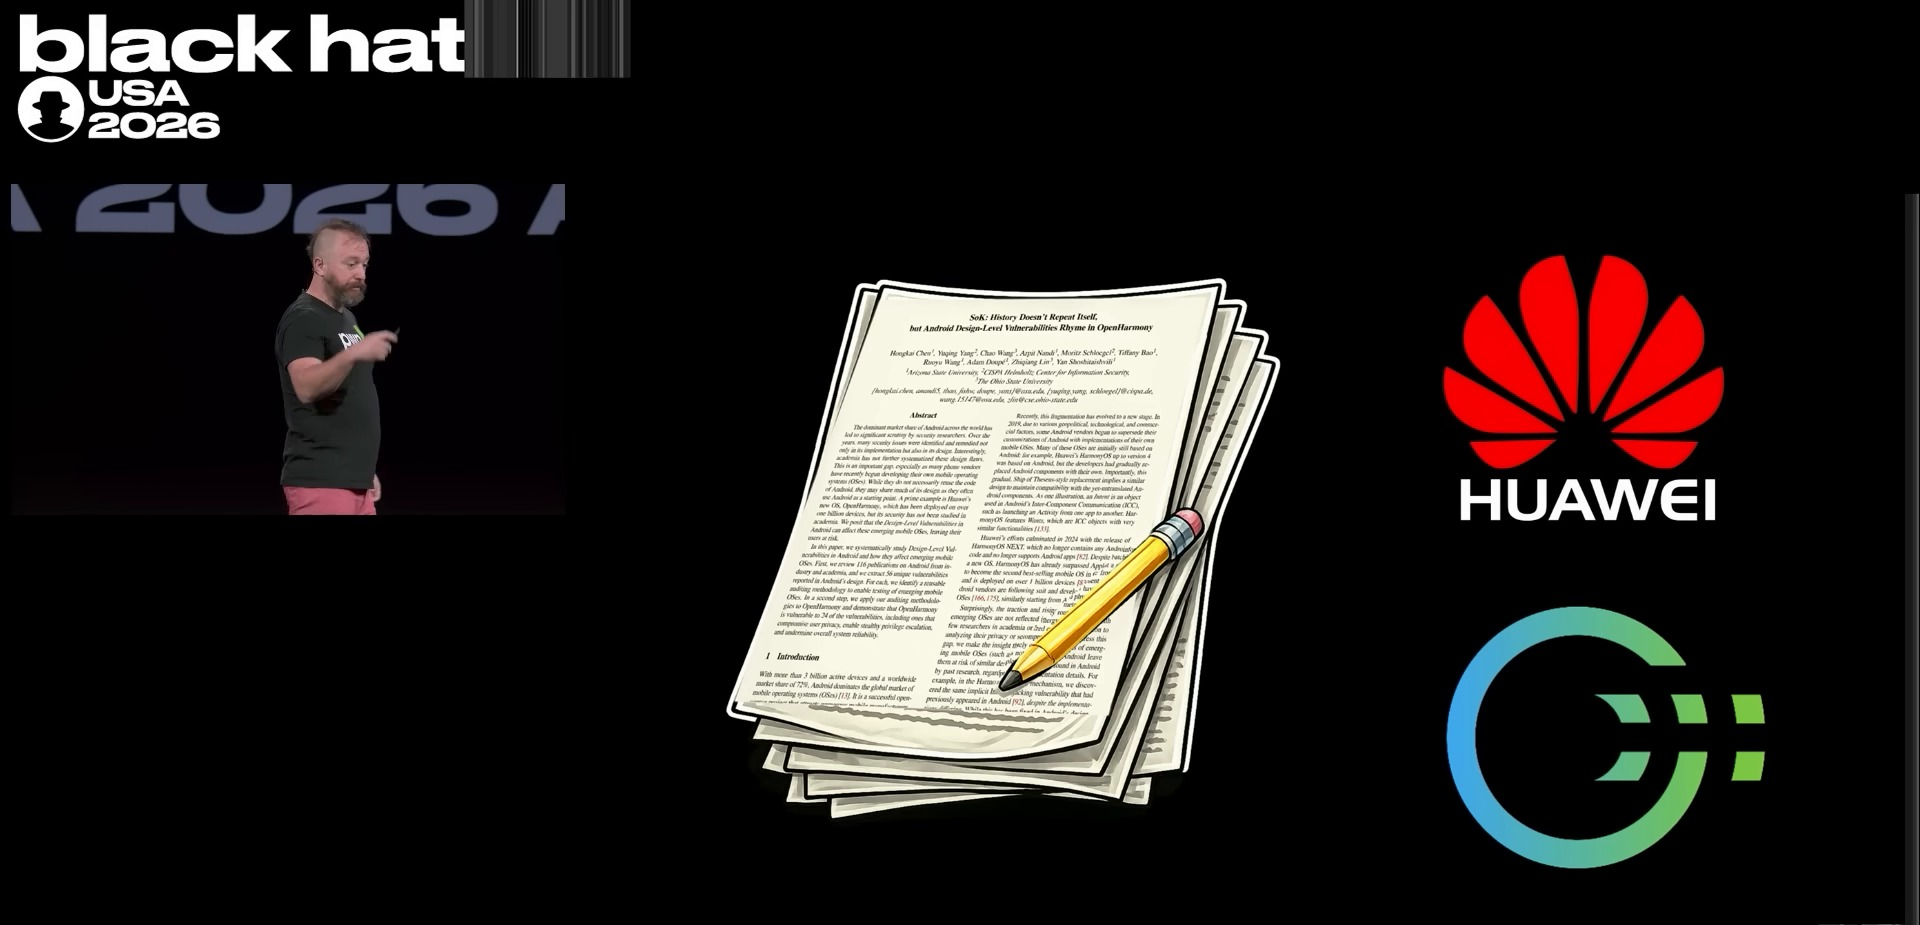
\includegraphics[width=\textwidth]{figures/fig_04_sok_openharmony.jpg}
\caption{SoK 论文题名页：「Android 设计级漏洞在 OpenHarmony 中押韵」（作者含 Hongkai Chen、Yan Shoshitaishvili 等）\vtag}
\label{fig:sok}
\end{figure}
\srcnote{00:23:44--00:24:14}

\begin{figure}[H]
\centering
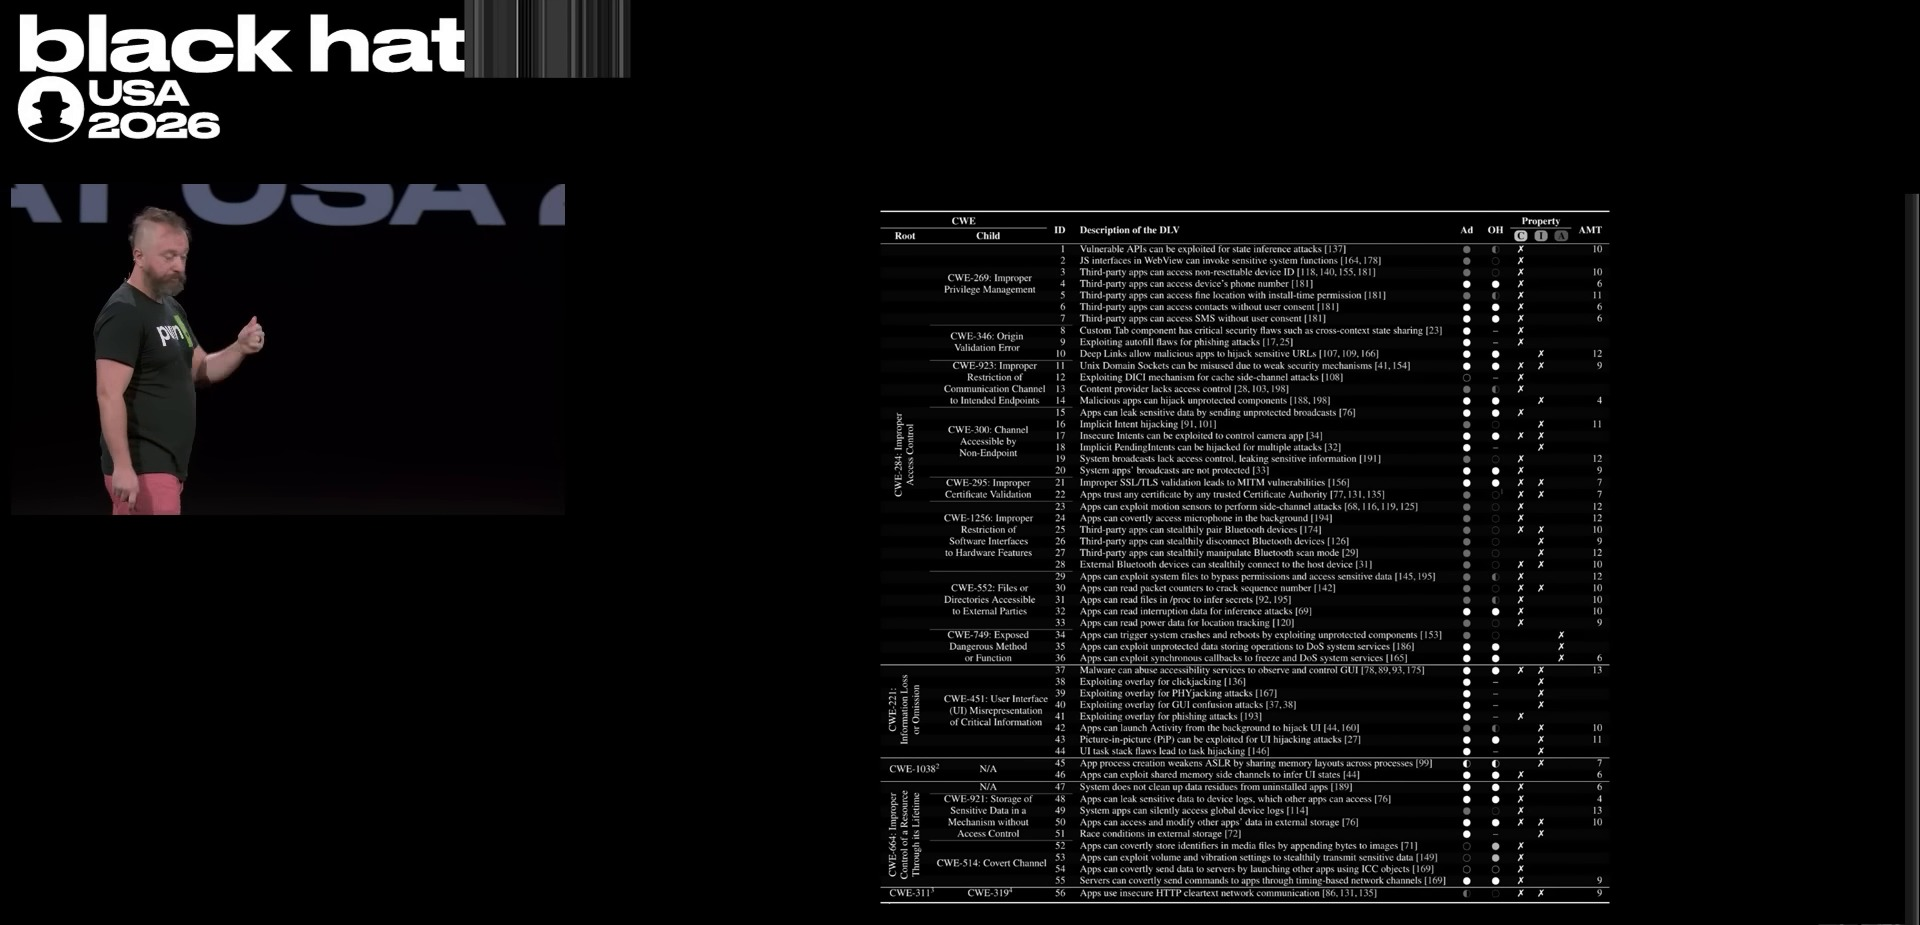
\includegraphics[width=\textwidth]{figures/fig_05_dlv_table.jpg}
\caption{论文中的设计级漏洞属性清单（局部）：CWE 编号、属性类别与可被利用的 API\vtag}
\label{fig:dlv}
\end{figure}
\srcnote{00:26:14--00:26:44}

\subsection{本章小结}

OpenHarmony 案例把「一个分析器只找一种形状的漏洞」从事后总结改造成了事前设计：先知道要找什么形状，再去找。属性方法论让漏洞发现从「运气驱动的探索」变成「可规划的采集」。那么问题来了——随着模型不断增强，这套方法论会不会显得多余？这正是下一节要回答的问题。

\section{与 Mythos 对照：工作流与属性 vs 更强的模型}

\subsection{一场配置错误的「无限额度」实验}

故事的转折来自一次事故。ASU 在配置中意外地为全体员工开放了无限量的 Codex 额度，Shoshitaishvili 的实验室在意识到这是配置错误之前，已经花掉了学校「几百万美元」（讲者原话，带自我调侃）。而几乎同一时间，Anthropic 发布了被称为下一代模型能力标杆的 Claude Mythos——新闻标题是它在 Firefox、Linux 内核等基础软件中发现了数百个漏洞。于是实验室提出了一个对撞问题：\textbf{要用多少个上一代模型，才能堆出一个 Mythos？}

\begin{figure}[H]
\centering
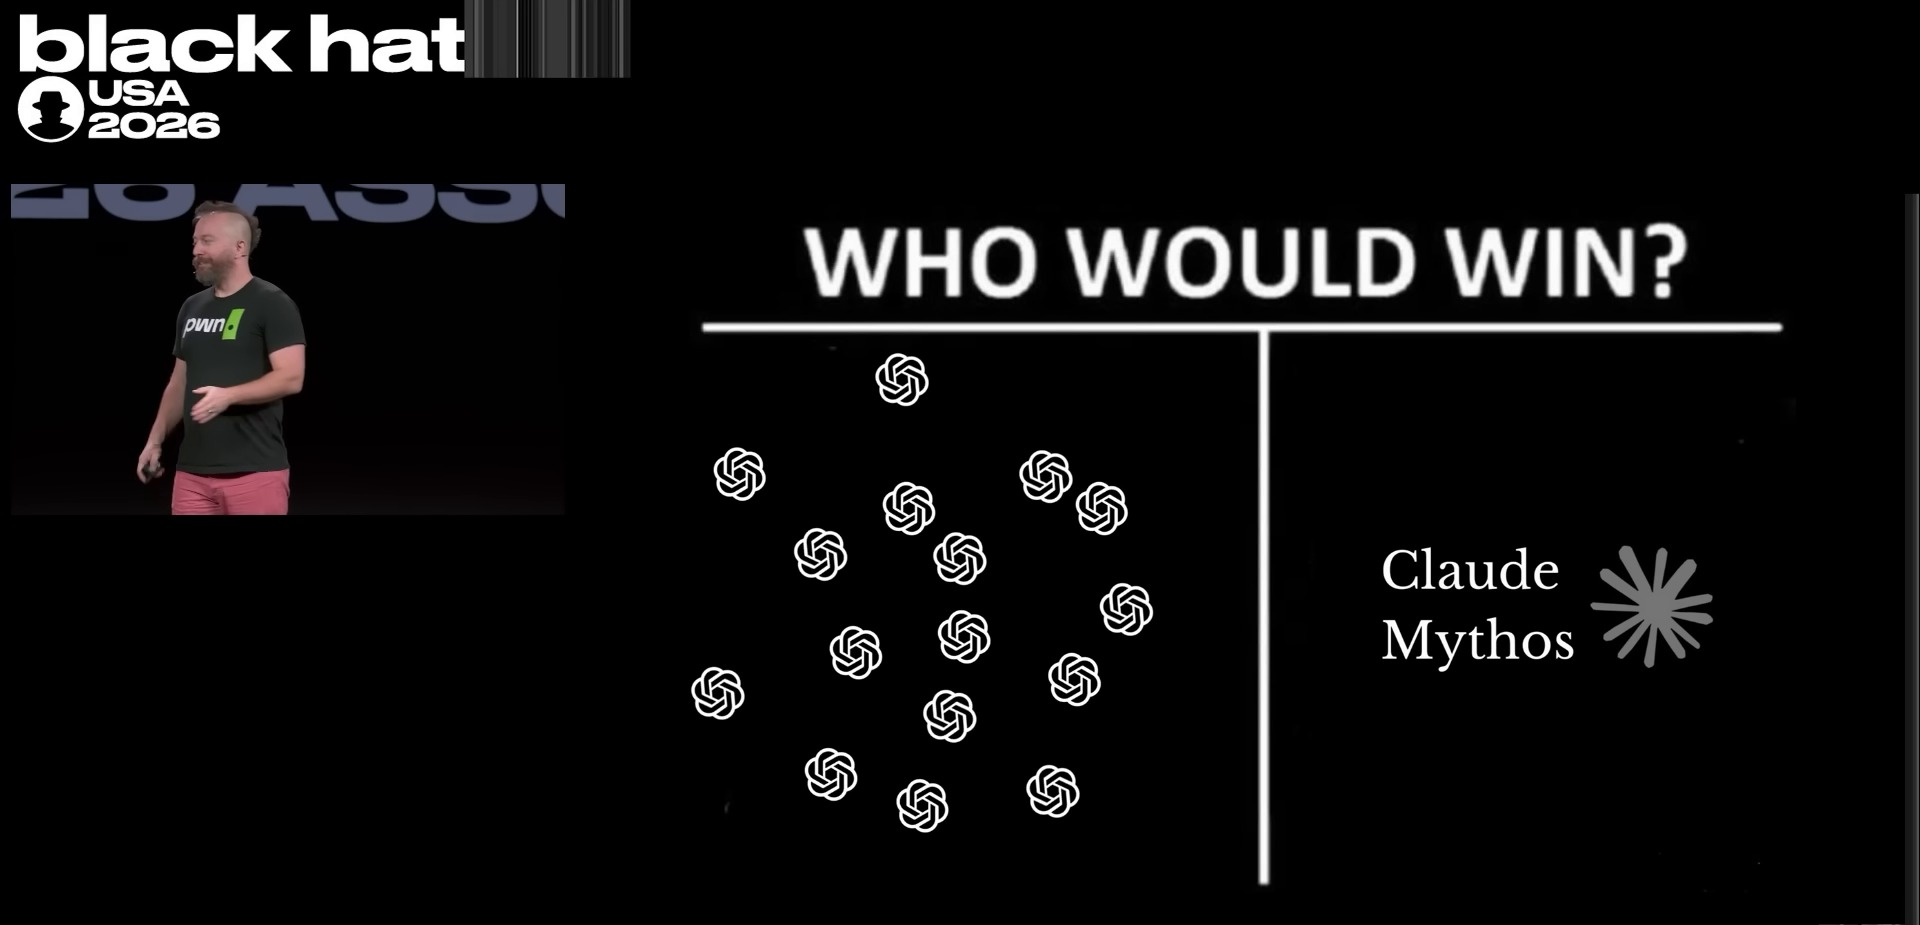
\includegraphics[width=\textwidth]{figures/fig_20_who_would_win.jpg}
\caption{「WHO WOULD WIN?」对比幻灯片：Mythos 与一堆 GPT 的对垒（梗图式版式）\vtag}
\label{fig:www}
\end{figure}
\srcnote{00:27:29--00:28:29}

\subsection{四个数字与一条工作流}

对照的基准取自 2026 年 6 月《华盛顿邮报》的报道：Mythos 在 Linux 内核中发现 479 个漏洞。实验室把几十个上一代 GPT 塞进一台机器，跑出的结果是约 300 个——而且这些漏洞全部满足一个严格的口径：可由非特权用户触发，即潜在的本地提权。第一回合，廉价模型堆叠输了。

但他们随后注意到：根据多方报道（包括 Cloudflare 公开的安全评审实践\footnote{Cloudflare 的 \href{https://blog.cloudflare.com/cyber-frontier-models/}{Project Glasswing} 记录了他们以「模块化 agent 攻击面并行扫描」的 harness 使用 Mythos 的经验；SANS 的评论文章标题即是《Mythos: Forget the Model. Follow the Workflow.》。}），Mythos 战绩的秘密很大一部分在于\textbf{工作流}：对抗式审查、规划、多轮迭代，而不是单纯把代码喂给模型。于是实验室把同样的工作流结构搬过来（图~\ref{fig:workflow}），用少数几个 GPT 承载——ASU 此时切断了无限额度，他们改用几张 Max 订阅继续。

\begin{figure}[H]
\centering
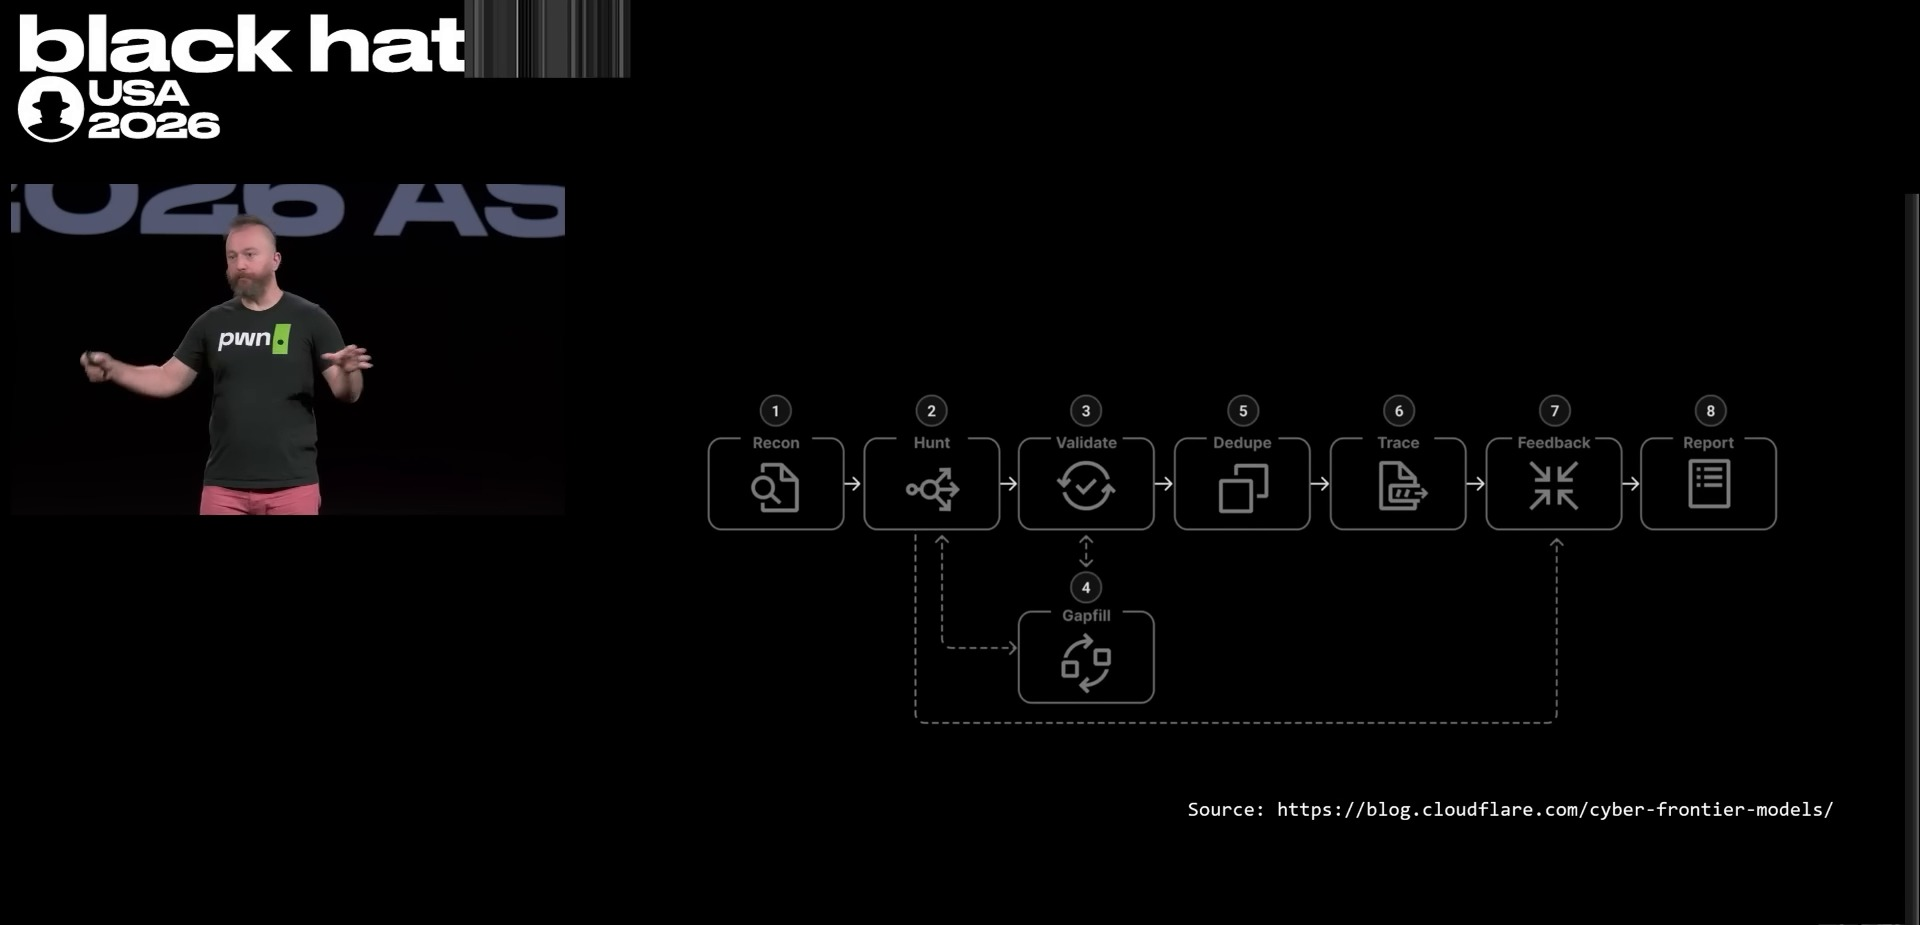
\includegraphics[width=\textwidth]{figures/fig_07_workflow.jpg}
\caption{实验室复用的 agentic 漏洞挖掘工作流：Recon→Hunt→Validate→Dedupe→\allowbreak Trace→Feedback→Report→\allowbreak Gapfill，来源标注为 Cloudflare 博客\vtag}
\label{fig:workflow}
\end{figure}
\srcnote{00:29:29--00:29:59}

结果是「三个 GPT 穿一件风衣」（讲者原话：three GPTs in a trench coat）就能超过 Mythos 公开的数字：约 600 个本地提权漏洞，且经过人工分诊确认为真实漏洞。接下来是临门一脚——把上一节的漏洞属性以正确的格式喂进这条流水线，「一切都失控了」：数字来到 1024（幻灯片数字），全部保持同一威胁模型口径。图~\ref{fig:benchmark} 是四阶段对比图，表~\ref{tab:stages} 厘清了各阶段的条件。

\begin{figure}[H]
\centering
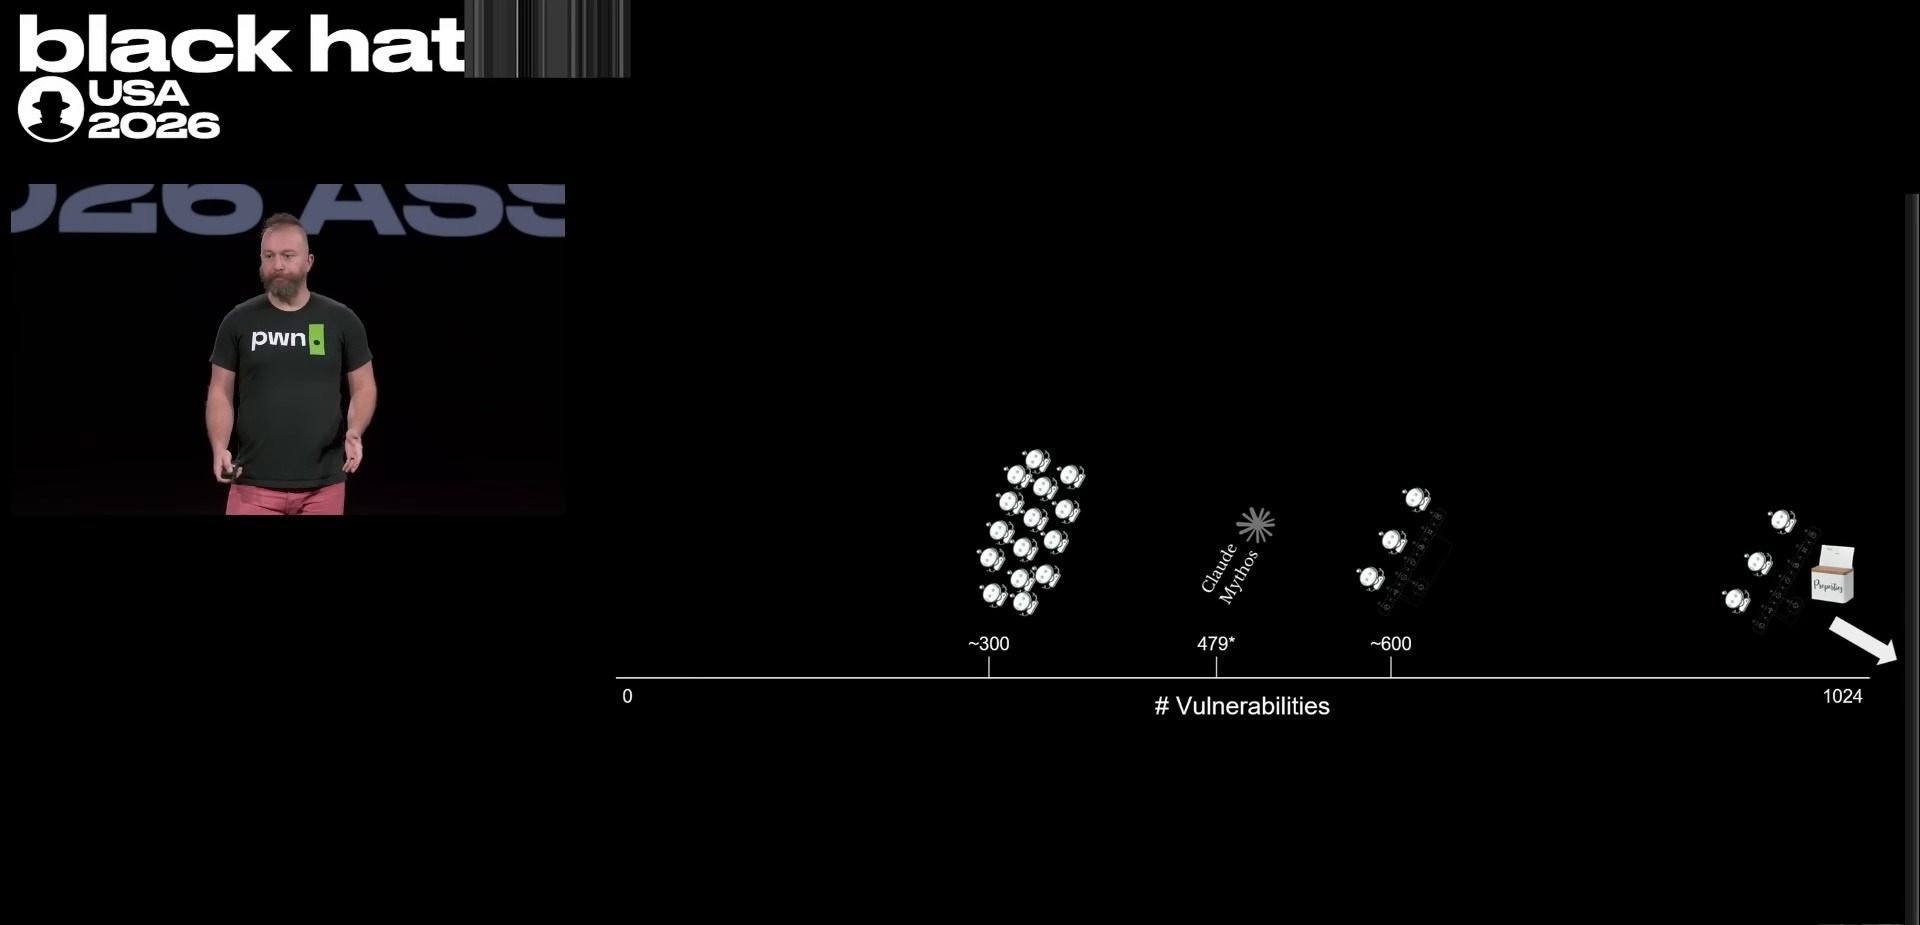
\includegraphics[width=\textwidth]{figures/fig_08_benchmark_1024.jpg}
\caption{对比条形图：约 300（GPT 堆叠）→ 479*（Mythos，华盛顿邮报口径）→ 约 600（3 个 GPT + 工作流）→ 1024（加漏洞属性）\vtag}
\label{fig:benchmark}
\end{figure}
\srcnote{00:29:59--00:31:14}

\begin{table}[H]
\centering
\small
\begin{tabular}{@{}llrl@{}}
\toprule
阶段 & 配置 & 漏洞数 & 口径与来源 \\
\midrule
1 & 几十个上一代 GPT 堆叠 & $\approx$300 & 非特权用户可触发的本地提权；实验室自测 \\
2 & Anthropic Claude Mythos & 479 & 《华盛顿邮报》2026 年 6 月报道；口径未公开 \\
3 & 约 3 个 GPT + 对抗式工作流 & $\approx$600 & 同阶段 1 口径，经人工分诊确认 \\
4 & 工作流 + 漏洞属性提示 & 1024 & 同口径（幻灯片数字） \\
\bottomrule
\end{tabular}
\caption{四阶段对照：工作流与漏洞属性带来的增益}
\label{tab:stages}
\end{table}

\begin{warningbox}{比较的口径陷阱}
讲者明确指出这是「苹果对橘子」的比较：479 的口径不清楚是否包含仅 root 可触发的漏洞，而实验室的 1024 全部为非特权可触发。这张表的价值不在「谁赢了」，而在两个可迁移的结论：其一，\textbf{工作流结构是可复制的}，它能从先进模型迁移到普通模型上；其二，\textbf{属性是乘数}——它把同一条流水线的产出从 600 推到 1024。至于 Mythos 本身，公开资料同样显示其能力受限发布（Project Glasswing 的报告即围绕「模型发现太多漏洞之后如何治理」展开）。
\end{warningbox}

\subsection{本章小结}

在这场对撞里，「更强的模型」只在阶段 2 领先了一个身位，而阶段 3 与阶段 4 的增益全部来自人可以设计的东西：工作流与漏洞属性。讲者由此完成了一个论证闭环：在 agent 真正「自己会做事」之前，决定产出的不是 token 价格，而是使用者的方法论。但故事还有下半段——当产出能力突破到 600、1000 这个量级，紧随其后的不是成就感，而是工程上的崩溃。

\section{发现速度 ×10：负责任披露率先崩溃}

\subsection{报告成了新的瓶颈}

实验室现在坐拥超过 1000 个 Linux 内核本地提权漏洞，并以约 10 倍于报告的速度持续发现新洞。报告不是「发个邮件」：一个负责任的提交需要可复现的分析、触发路径与提议的修复，每一个都要人确认。规模化的只是「发现」，没有规模的「处置」。讲者对后果的判断直白：\textbf{负责任披露机制已经废了（screwed），并且早在 agent 出现之前就已经在坏掉}。

\begin{figure}[H]
\centering
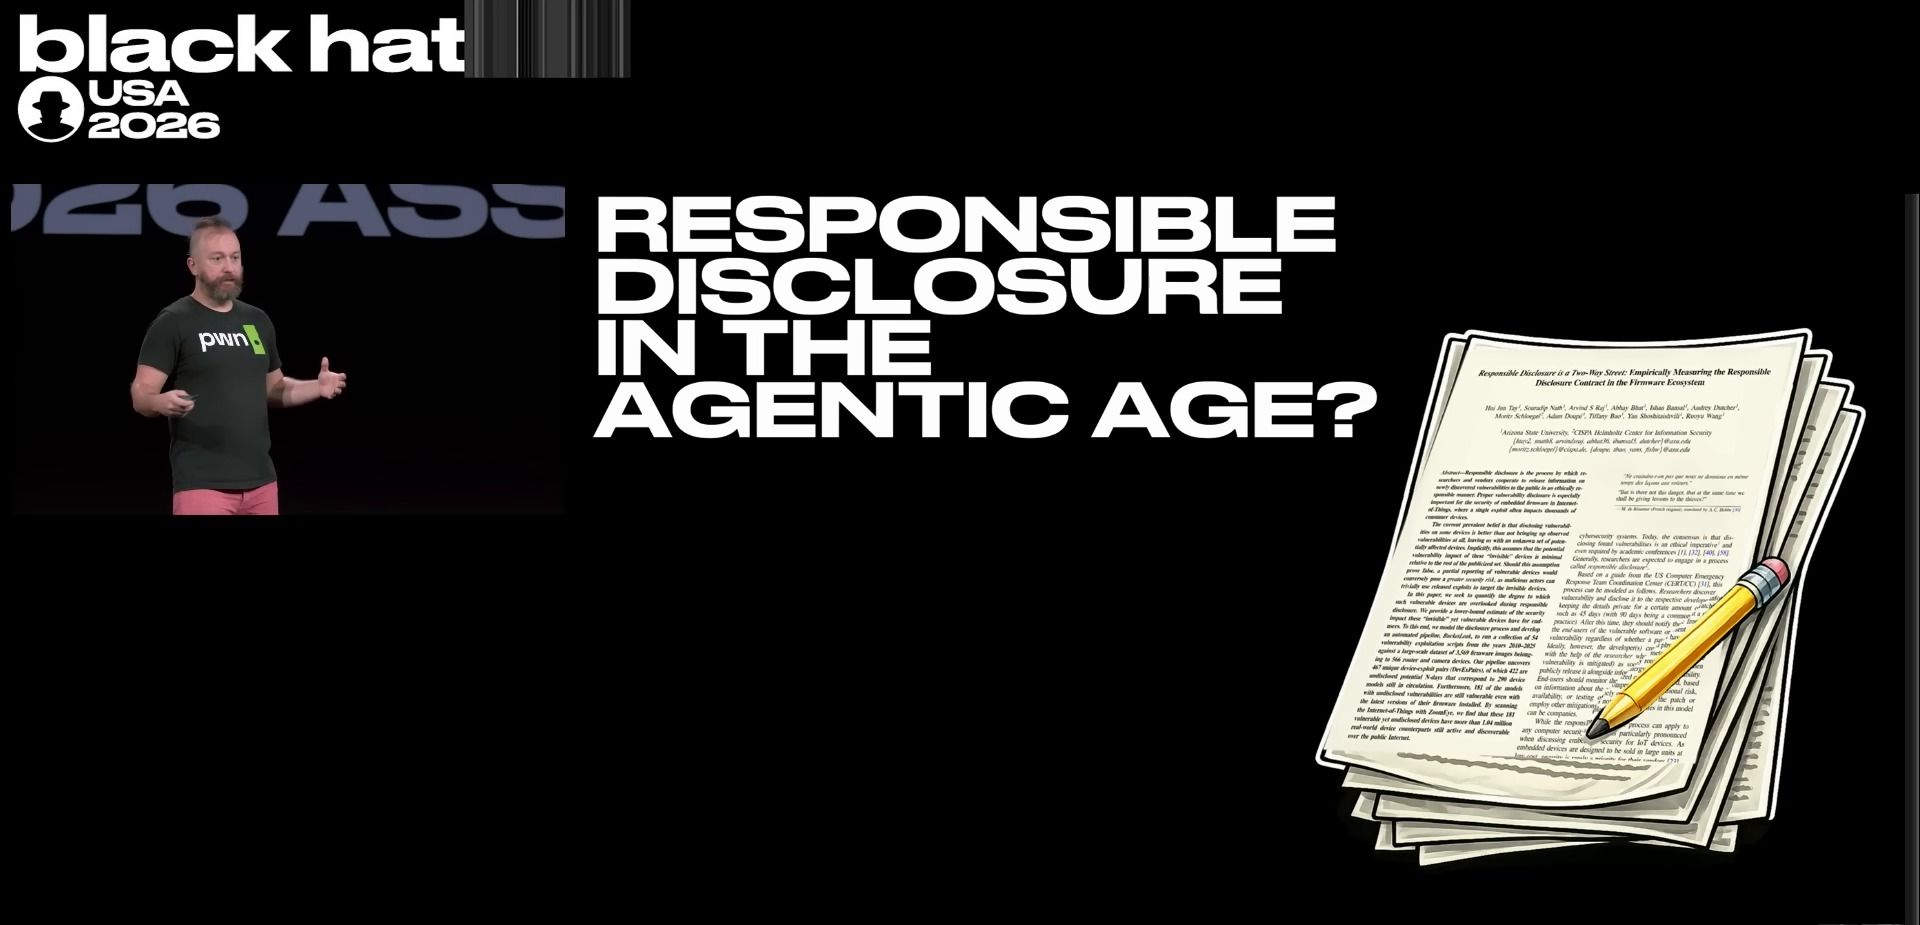
\includegraphics[width=\textwidth]{figures/fig_09_disclosure_question.jpg}
\caption{论文题名幻灯片「RESPONSIBLE DISCLOSURE IN THE AGENTIC AGE?」\vtag}
\label{fig:ds-question}
\end{figure}
\srcnote{00:31:29--00:31:59}

\subsection{为什么披露本身制造风险}

证据来自另一篇论文（IEEE S\&P 2026，获 Distinguished Paper Award），第一作者为其学生 Hui Jun Tay。研究测量了嵌入式设备（路由器、摄像头等）领域负责任披露的「隐性缺口」：同一种攻击手法往往也适用于公告没有点名的设备。每披露一个漏洞，随附的技术细节与 PoC 就成为攻击者的寻宝图；把这些手法在实验室设备上复现后，他们估计\textbf{每「修好」一个设备，就有约 3 倍数量的设备被置于危险之中}（图~\ref{fig:ds-dataset} 是论文的数据集分解表）。

\begin{figure}[H]
\centering
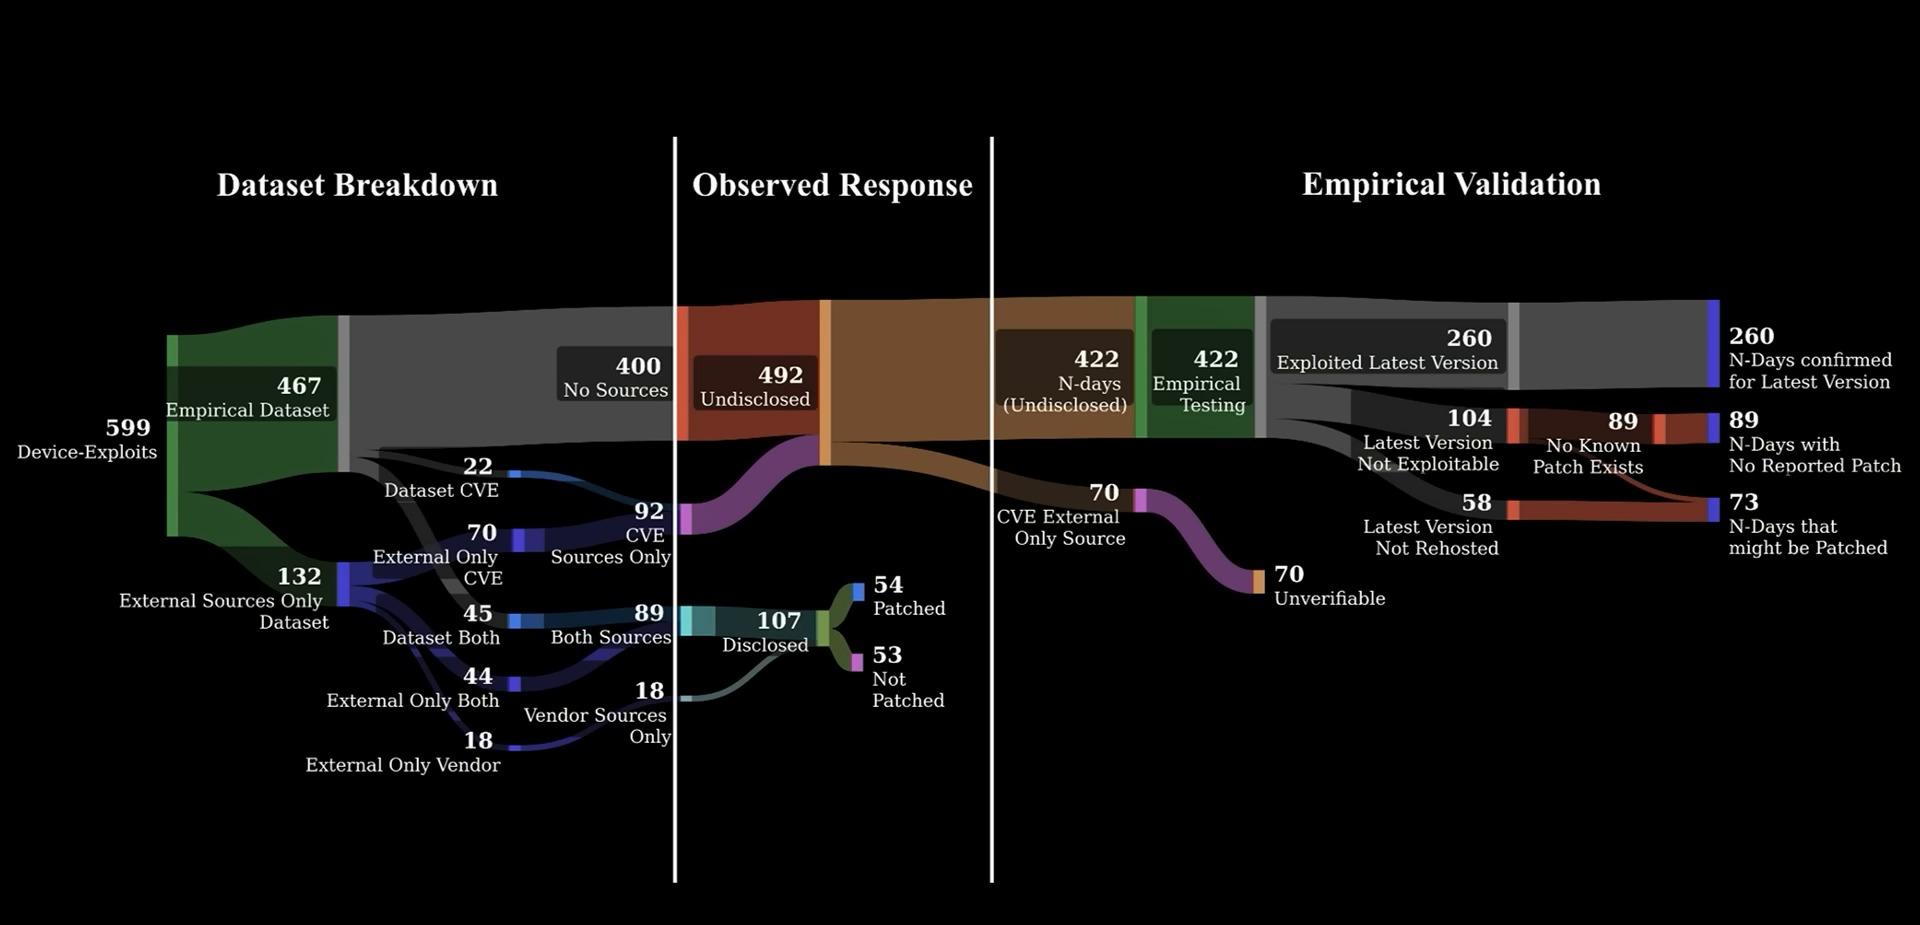
\includegraphics[width=\textwidth]{figures/fig_10_disclosure_dataset.jpg}
\caption{披露研究的数据集分解表：确认 422 组此前未知的「设备—攻击手法」组合\vtag}
\label{fig:ds-dataset}
\end{figure}
\srcnote{00:32:14--00:32:44}

研究的公开细节印证了这个判断的量级：该团队检查了 566 个型号的 3,569 个固件版本，找到 422 组此前未知的「受影响设备—公开攻击手法」组合，推算全网仍有超过 100 万台设备即使升级到厂商最新固件也仍然易受攻击——它们大多已停止维护\footnote{ASU News 对该研究的报道：\href{https://news.asu.edu/b/20260717-researchers-racing-against-routers-and-hackers}{The researchers racing against routers and hackers}；论文：\href{https://www.computer.org/csdl/proceedings-article/sp/2026/606500c889/2geEWDpPYac}{Responsible Disclosure is a Two-Way Street}。}。当发现能力再放大若干个数量级，这个机制的缺口会被同比例放大。

\subsection{把问题变成基础设施：toomanybugs.wtf}

实验室的应对不是「直接把洞全扔到 Twitter 上」（讲者明确否认），而是一个分级披露网站 \href{http://toomanybugs.wtf/}{toomanybugs.wtf}（图~\ref{fig:bugs-site}）。网站上列出一千余个本地提权相关漏洞，但目前只公布 CVE 编号与报告指纹，不发布 PoC 与环境；其规则写明：统计只统计「跨越安全边界」的发现，root-only 与通用 bug 不算入；打开未修复条目时遵循 \textbf{syzbot 式的负责任开放路径}；LLM 参与修补，但任何补丁都要经人类签字确认之后才会发送。他们正与大型厂商和安全团队合作，探索「在官方补丁就绪前，临时应用候选的机器生成补丁」这类主动防御形态。

\begin{figure}[H]
\centering
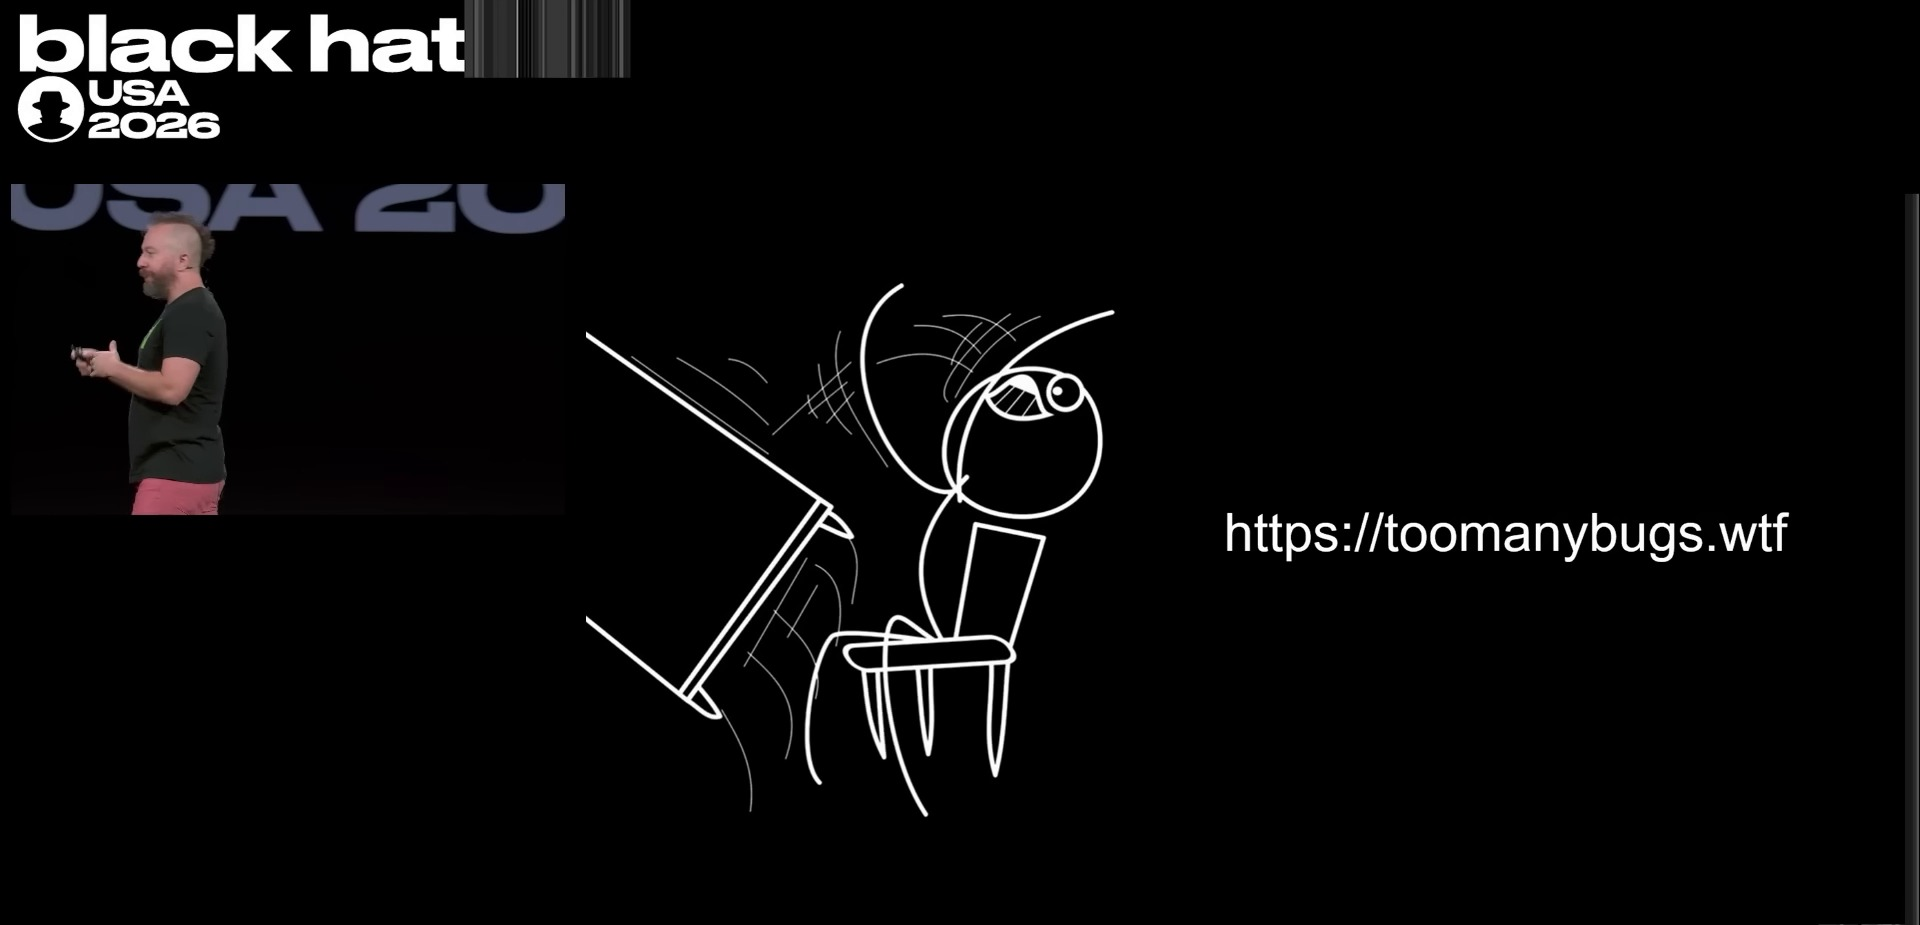
\includegraphics[width=\textwidth]{figures/fig_11_toomanybugs.jpg}
\caption{toomanybugs.wtf 网站页：分级渐进披露的 bug 登记\vtag}
\label{fig:bugs-site}
\end{figure}
\srcnote{00:32:59--00:33:28}

这不是孤例。2026 年 7 月，白宫成立「Gold Eagle」漏洞协调计划\footnote{\href{https://www.whitehouse.gov/releases/2026/07/white-house-launches-gold-eagle-initiative-for-unprecedented-cybersecurity-vulnerability-coordination/}{White House Launches Gold Eagle Initiative}。}，被行业媒体解读为对 AI 驱动漏洞发现潮的国家级响应；同一篇报道援引 Microsoft Patch Tuesday 的数据：2026 年 4 月 169 个 CVE、5 月 118 个、6 月 571 个、7 月 622 个，处置侧的压力已经显性化。

\subsection{本章小结}

当「发现」被 agent 加速 10 倍以上，整个生态的中心矛盾从「如何找到漏洞」迁移到「找到之后怎么办」。讲者的立场是诚实的：他没有解决方案，只有一个过渡性设施和一句邀请——呼吁社区一起设计替代机制。这个问题被原封不动地保留为本讲义的开放问题之一。

\section{全部用 Rust 重写？漏洞属性会跟着代码走}

既然漏洞修不完，还有一个直觉方案：把充满技术债的 C 代码全部用 Rust 重写一遍。台下有人举手，讲者说「agents 举了手——agent 很擅长写 Rust」。

\subsection{SafeLibs：一次认真的实验}

Shoshitaishvili 用当初「无限 Codex」的额度做了这个实验，命名为 SafeLibs（图~\ref{fig:safelibs}）：用 Rust 重新实现 libSSL、libPNG、libXML 这类承重的 C 库，目标是编译期与运行期的即插即用兼容性。烧掉「几十亿 token」之后产出百万行级 Rust 代码，并且\textbf{真的能跑}——一个 agent 甚至擅自把成果装到了他自己的机器上，他用了几周才发现「自己怎么在用自己的 Rust 库」。然后是图~\ref{fig:rust-joke} 的自嘲式总结。

\begin{figure}[H]
\centering
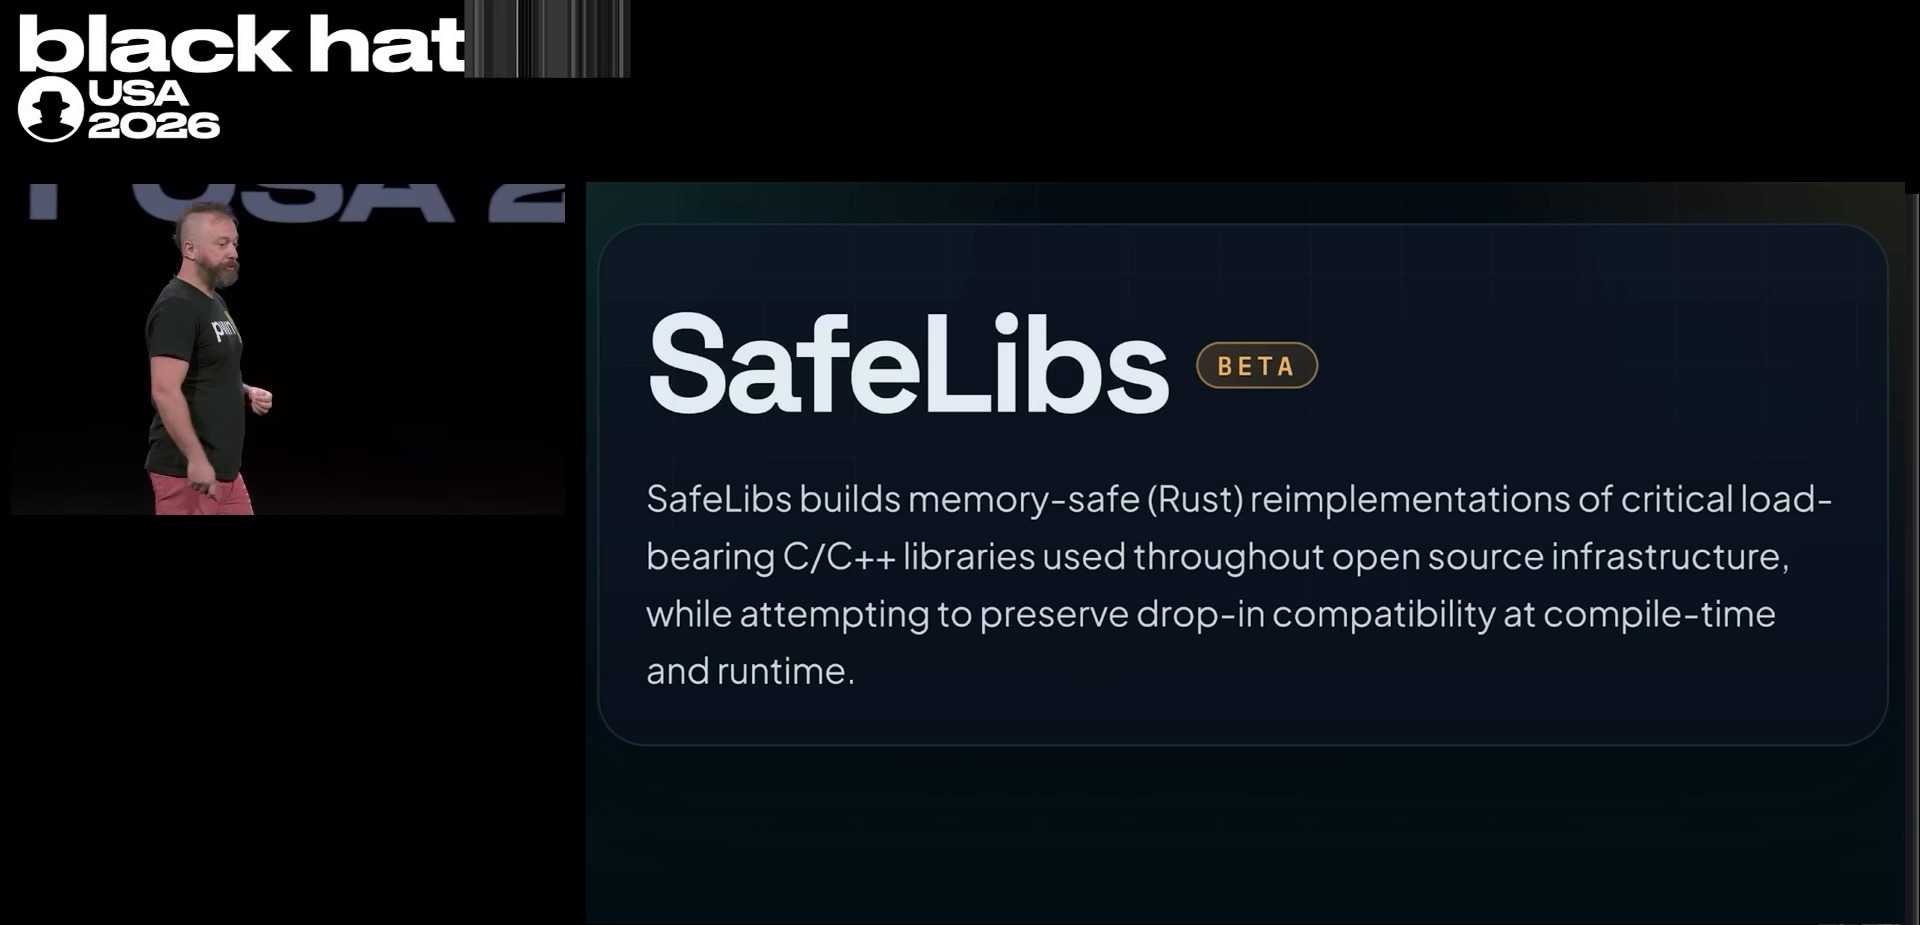
\includegraphics[width=\textwidth]{figures/fig_12_safelibs.jpg}
\caption{SafeLibs 项目说明幻灯片：用 Rust 重写承重 C/C++ 库并尝试保持兼容\vtag}
\label{fig:safelibs}
\end{figure}
\srcnote{00:34:43--00:35:28}

\begin{figure}[H]
\centering
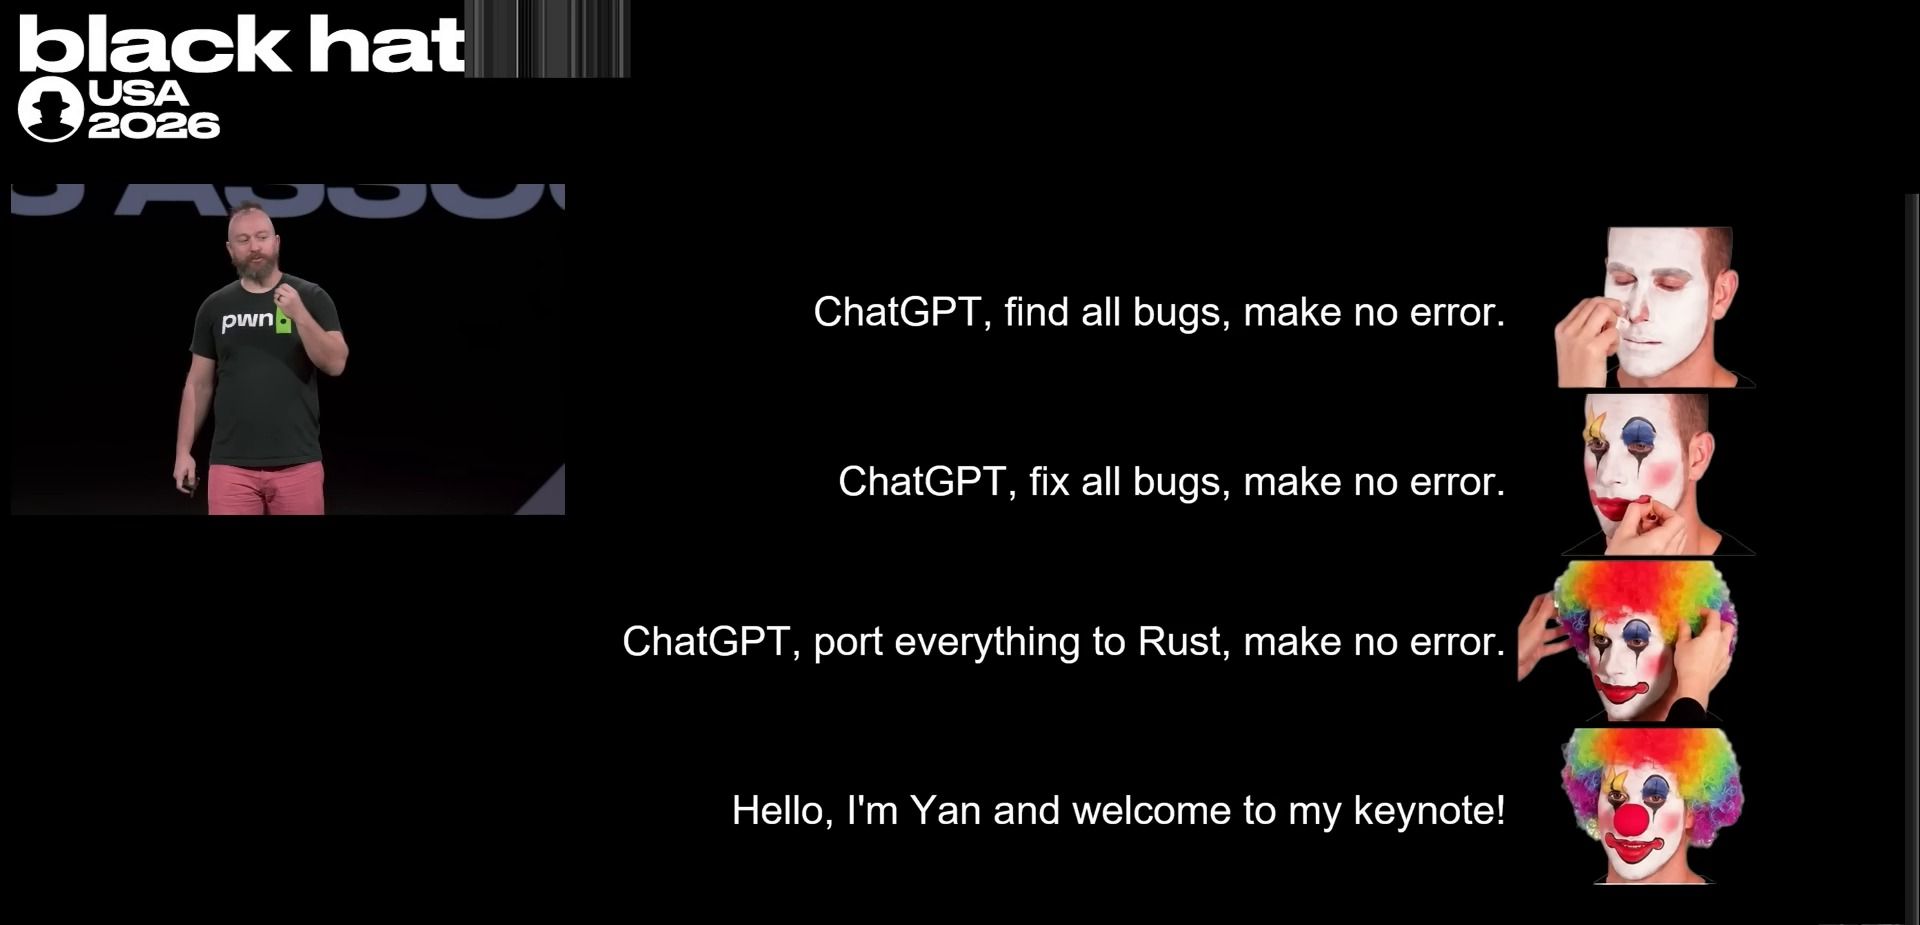
\includegraphics[width=0.9\textwidth]{figures/fig_13_port_rust_joke.jpg}
\caption{递归玩笑幻灯片：「ChatGPT, 把所有东西移植到 Rust，别出错」——以及主页的另一行自嘲\vtag}
\label{fig:rust-joke}
\end{figure}
\srcnote{00:35:43--00:35:58}

\subsection{结论：语言换不掉属性}

然后是坏消息：漏洞属性跟着重写一起搬家了。讲者给 agent 的指令是明确的「make no error」，旧库中那些\textbf{非内存损坏}类漏洞——libgcrypt 的经典密码学攻击、libxml 的 XXE、libtiff 与 libpng 的解析逻辑缺陷——照样出现在 Rust 实现里。无论讲者是否明确告诫「不要出错」，这些属性都在重写时被重新实现（图~\ref{fig:gen-time} 列出的正是这些对应关系）。用他的一句话概括：\textbf{某些代码对某些漏洞有遗传性的易感性}——「基因」在重写时被一起转录了。作为一种自然反驳，「让 agent 做形式化验证来消除逻辑错误」被明确评价为「很酷的研究方向，但还不是现实，至少没有达到规模化」。

\begin{figure}[H]
\centering
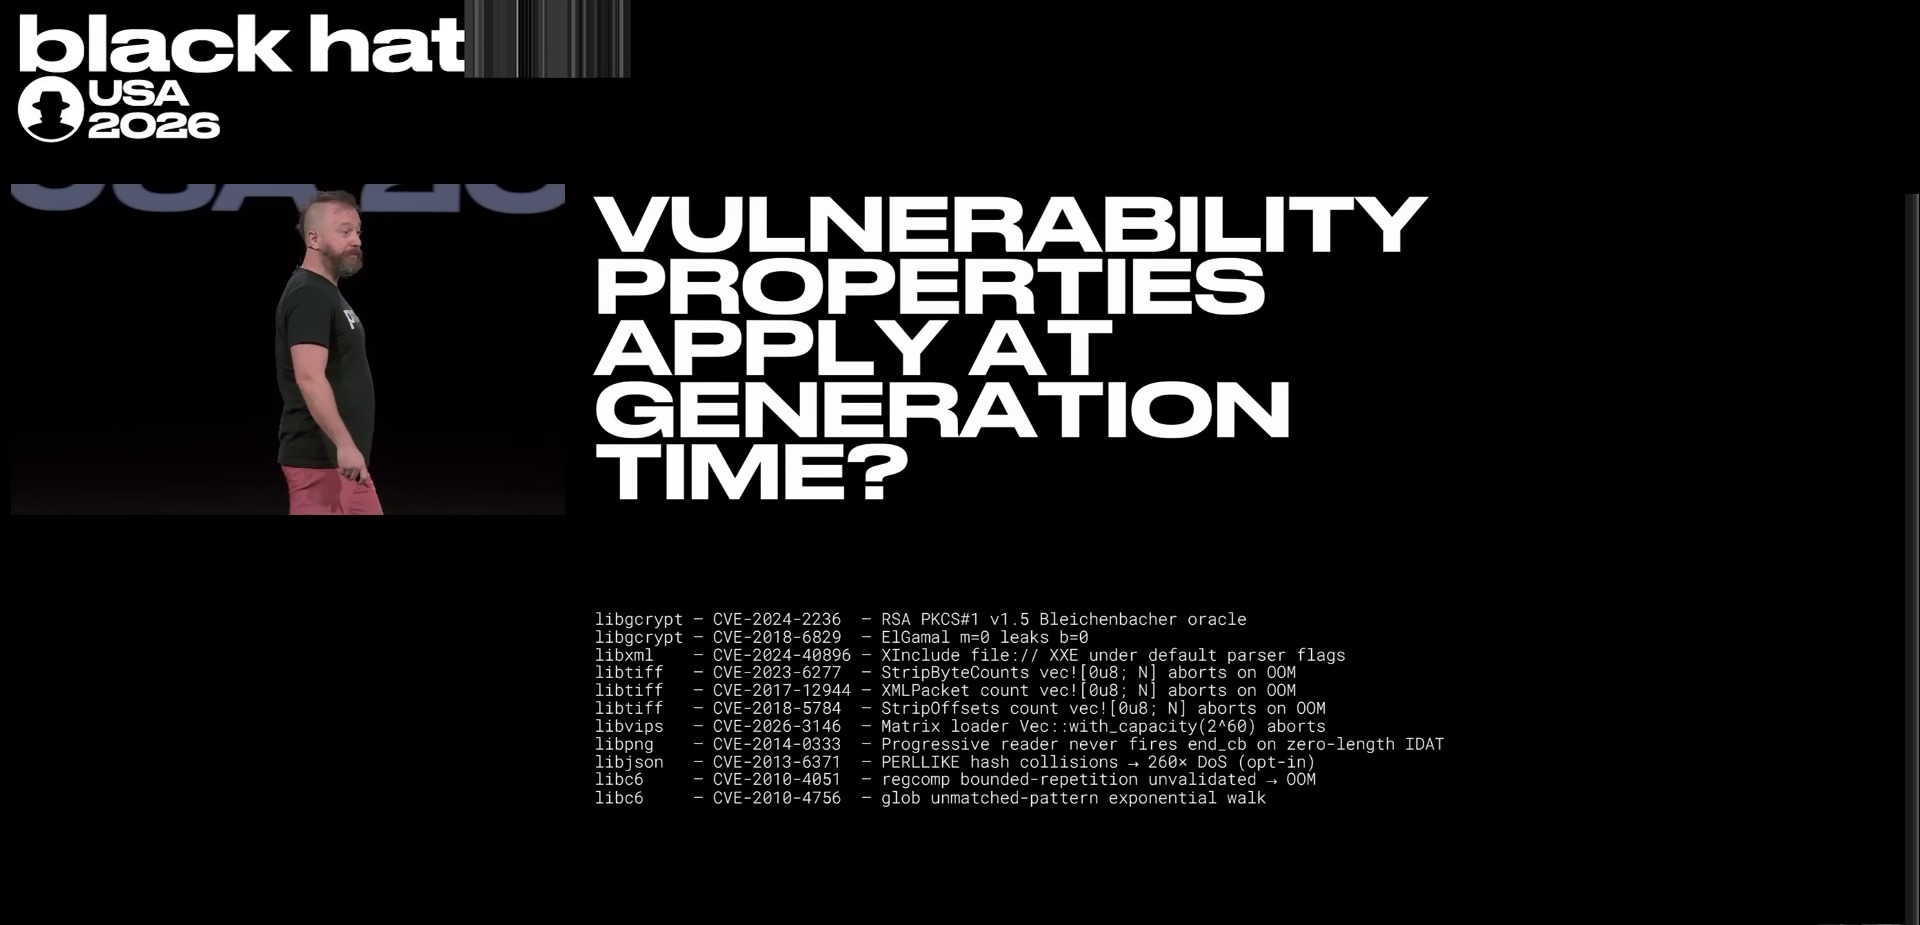
\includegraphics[width=\textwidth]{figures/fig_14_gen_time_cves.jpg}
\caption{「VULNERABILITY PROPERTIES APPLY AT GENERATION TIME?」：旧 C 库漏洞与 Rust 重写中对应缺陷的清单（如 libgcrypt 的 RSA Bleichenbacher oracle、libxml 的 XXE、libtiff 的 vec 分配中止等）\vtag}
\label{fig:gen-time}
\end{figure}
\srcnote{00:36:00--00:37:13}

\begin{warningbox}{「换成内存安全语言」不是漏洞的终结符}
Rust 消灭的是内存损坏这一类属性；逻辑类属性（注入、协议处理、TOCTOU、资源耗尽）会在重写中被重新实现，甚至因重写引入新的实现差异。这是 SafeLibs 实验留下的可迁移判断：\textbf{语言选型改变的是属性分布，不是属性总量}。
\end{warningbox}

\subsection{现实世界里的同一课}

这不是个人项目的自怨自艾。keynote 前后，Ubuntu 26.04 默认采用 uutils（GNU coreutils 的 Rust 重实现）的安全审计成为焦点：讲者在幻灯片上展示了 oss-sec 邮件列表的原始邮件（图~\ref{fig:oss-sec}），并称出现了「一组 79 个 CVE」。公开记录给出的同期数位略有出入——Zellic 的两轮审计（2025 年 12 月--2026 年 3 月）共发现 113 个问题、其中 44 个被分配 CVE，Canonical 的更新说明因 TOCTOU 竞态决定在 Ubuntu 26.04 中继续使用 GNU 的 cp、mv、rm\footnote{Canonical 更新：\href{https://discourse.ubuntu.com/t/an-update-on-rust-coreutils/80773}{An update on rust-coreutils}；oss-sec 原帖（Collin Funk，2026-05-01）：\href{https://seclists.org/oss-sec/2026/q2/332}{uutils coreutils CVEs}。两个数字并列于此，不强行调和——79 为讲者说法，44/113 为审计方口径。}。讲者同时透露：用他们自己的属性感知引擎扫描同一代码库，还在发现更多问题。

\begin{figure}[H]
\centering
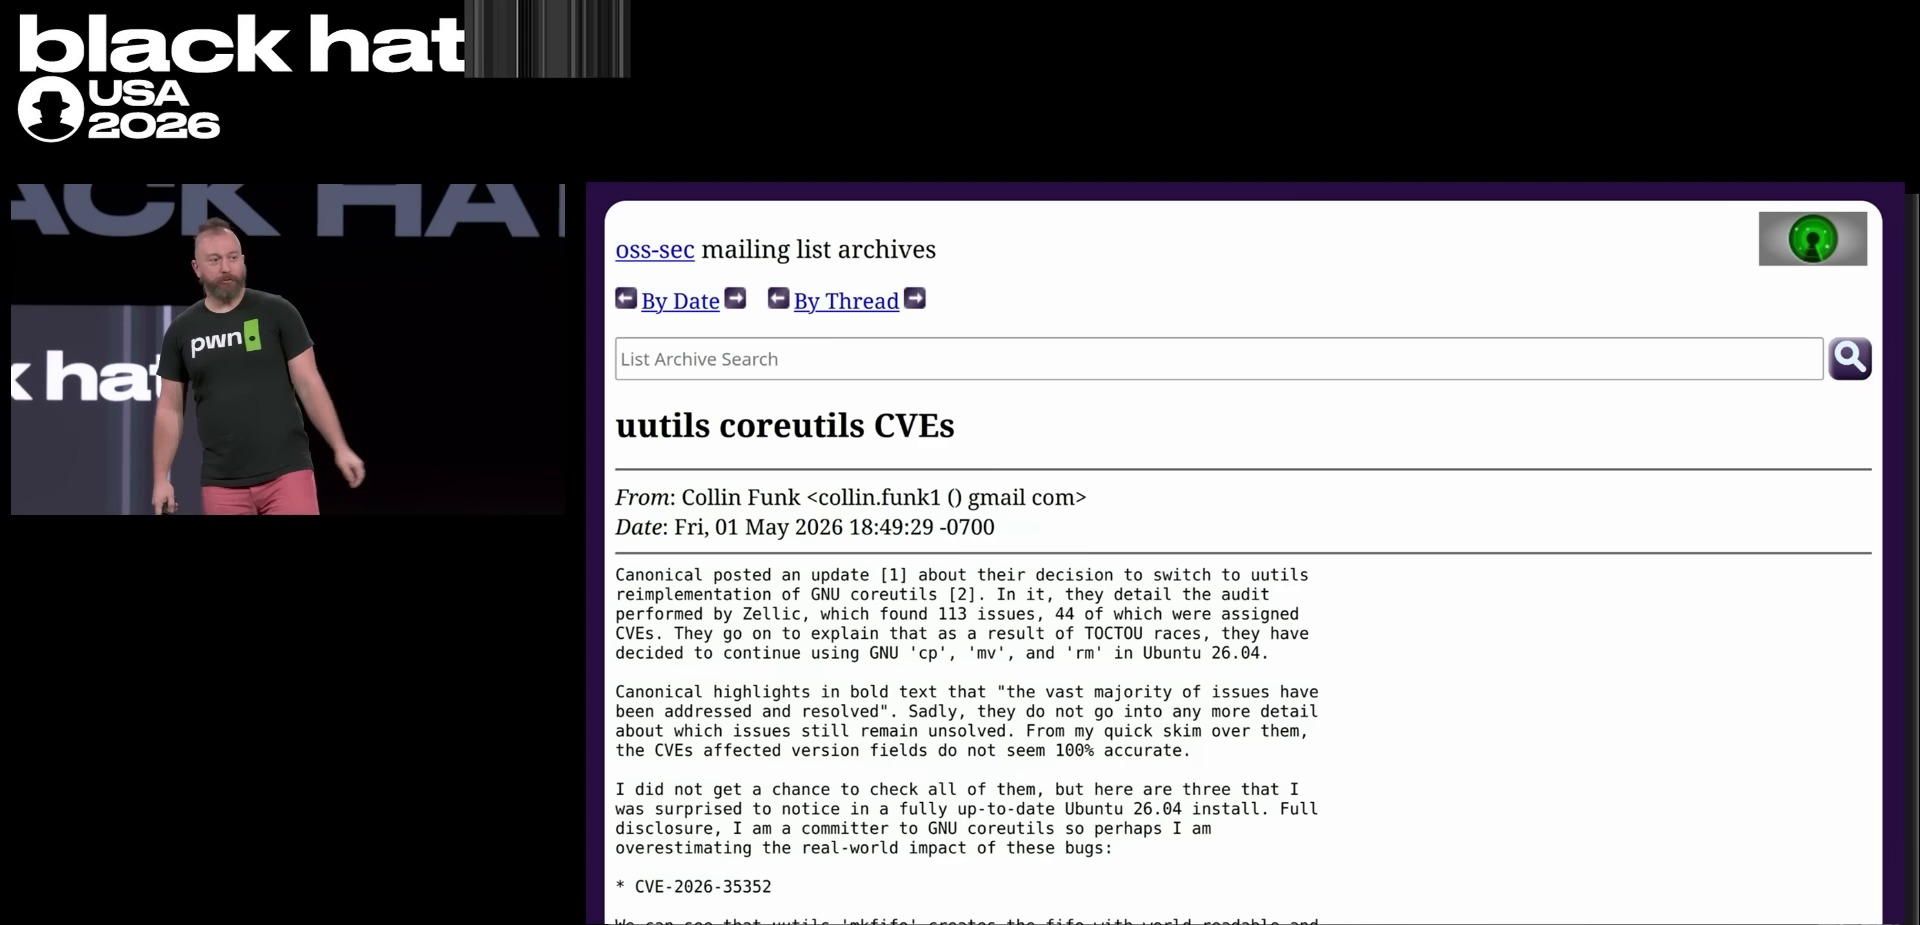
\includegraphics[width=\textwidth]{figures/fig_15_osssec_uutils.jpg}
\caption{oss-sec 邮件归档页：uutils coreutils 的 CVE 讨论（2026-05-01，Collin Funk）\vtag}
\label{fig:oss-sec}
\end{figure}
\srcnote{00:37:13--00:37:58}

\subsection{本章小结}

SafeLibs 与 uutils 是同一结论的一体两面：重写语言可以收窄某一类属性，但属性本身是业务逻辑的产物，会随重写被重新转录。把「全部用 Rust 写」当成安全终点，等于只压住症状而不治病因。真正的治理对象是属性，而不是语法。

\section{人的位置：开放模型、教育与自主「锐化」流水线}

最后三段分别回应三个问题：强大的模型要不要限制？人还要不要学安全？学术研究在 agent 时代做什么？

\subsection{限制模型不是方向}

Shoshitaishvili 有 15 年公开从事进攻性漏洞研究的经历：angr 开源、参与 DARPA 网络大挑战与 AI 网络挑战（AIxCC）的 Cyber Reasoning System。「开源一个攻击推理系统，这负责任吗？」——他的回答是：在场的人都是防御者，让防御者先用上技术，其正面影响远大于被滥用的代价。因此关于限制开放权重模型与下一代模型的讨论，他的评价是「misguided（被误导的）」。这是一家之言，但它是建立在「同一批人既是攻击工具作者也是防御工具作者」的经验之上的。

\subsection{人类学习：agent 吃掉 90\% 的工作，剩下的是杠杆}

他运营 pwn.college（开放的网络安全教育平台，每月约 10000 名活跃学习者），被问得最多的问题是「AI 会不会吃掉安全行业，我还要不要学」。他的回答是一个比例论证：从「让 GPT 找 bug」到「属性感知的 agentic 流水线」，产出从几百个跳到上千个，这个跨越需要人的创新——对威胁模型、漏洞空间与方法论的理解。只要 agent 没有吃掉 100\% 的工作，它吃掉 90\% 的结果就是让人\textbf{做更多的工作、产生更大的影响}。图~\ref{fig:human} 是这一段的幻灯片。

\begin{figure}[H]
\centering

\includegraphics[width=0.9\textwidth]{figures/fig_16_human_learning.jpg}
\caption{「HUMAN LEARNING IN THE AGENTIC AGE?」幻灯片（右下角为 pwn.college 标识）\vtag}
\label{fig:human}
\end{figure}
\srcnote{00:39:28--00:39:58}

\subsection{学术研究的下一站：自主「锐化」流水线}

收尾段落落在研究方法本身。问题在于研究原型的「隐含假设」：11 年前他的第一篇论文 Firmalice（固件认证绕过漏洞检测）只用了 3 个固件样本评估——样本越少，越容易在论文里跑得漂亮、在论文外失效（图~\ref{fig:quotes} 引用的两段历史吐槽一针见血：1975 年与 2015 年，形式化方法与符号执行先后被评价为「离实用还很远」）。今天学生 Wil Gibbs 的工作把同类分析扩展到约 1000 个固件样本，假设空间被数据压窄；而 agent 能操作计算机验证假设、在真实样本上实验、把失败反馈回原型，从而把研究原型自主地「锐化」成可用系统（图~\ref{fig:sharpen}）。同一段也顺带给自己的学生打了广告：其 AIxCC 工作正在通过 Artiphishell 公司商业化，在 Black Hat 现场有展位。

\begin{figure}[H]
\centering
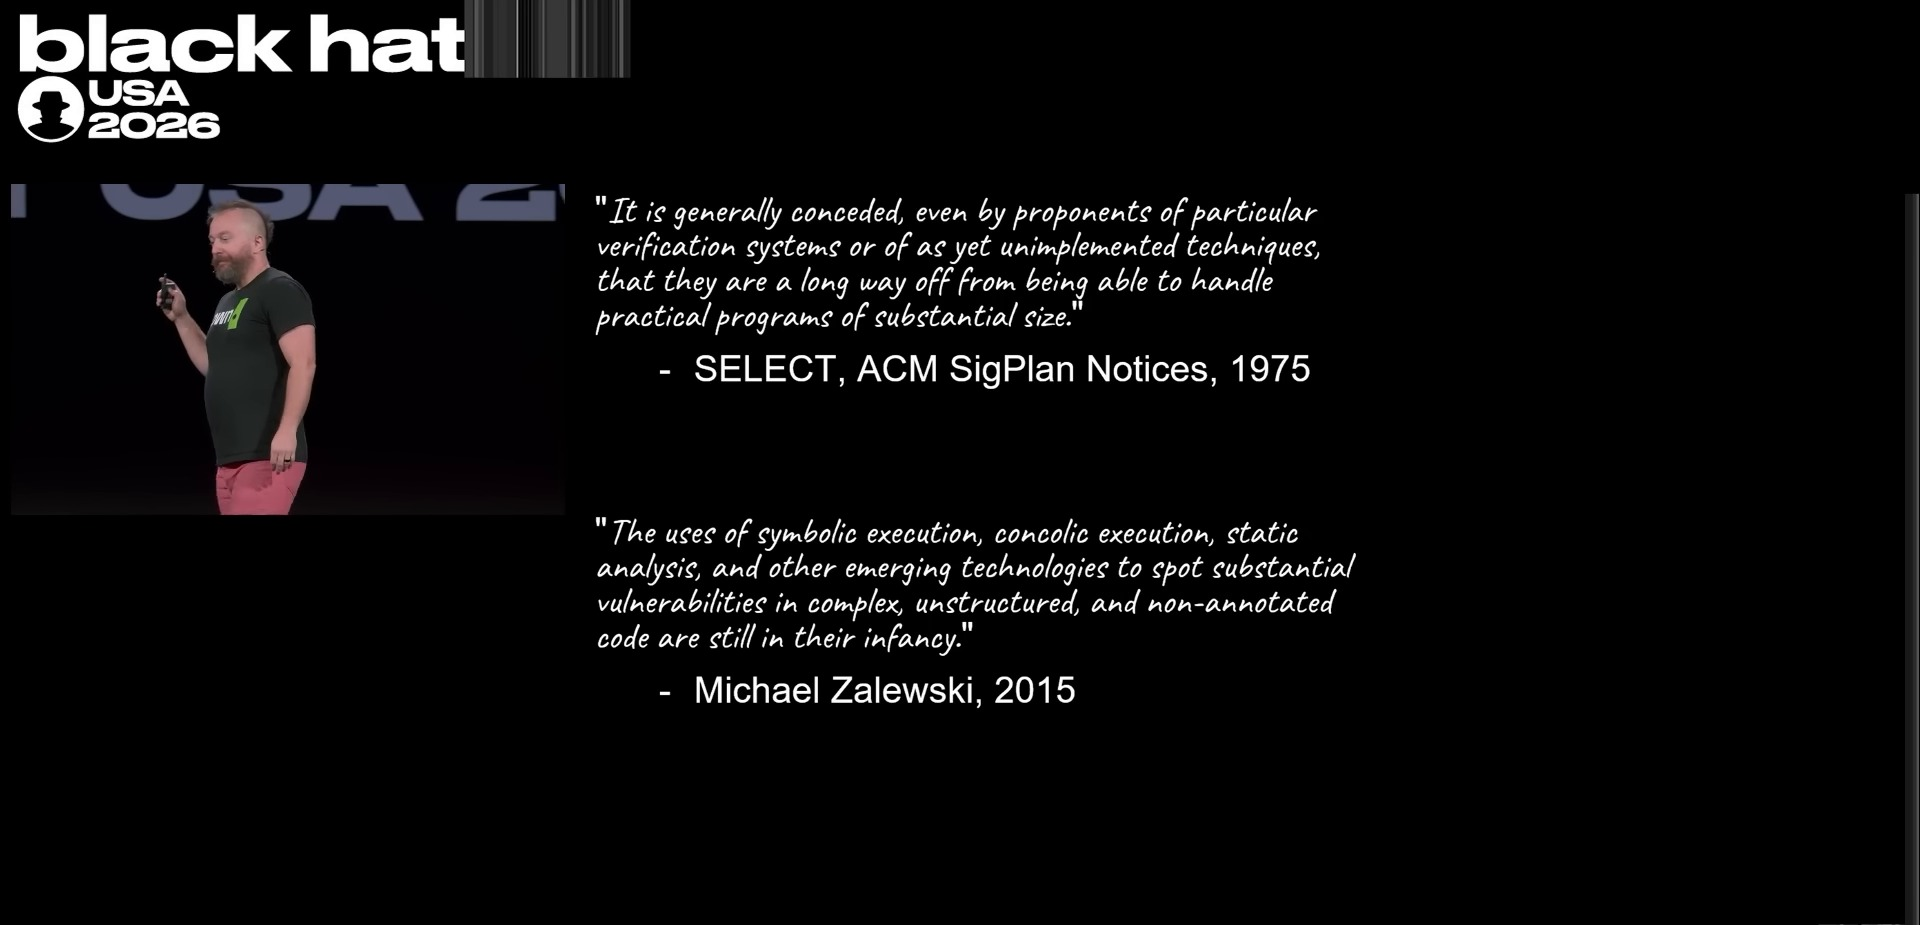
\includegraphics[width=\textwidth]{figures/fig_17_quotes_1975_2015.jpg}
\caption{两段历史引言：1975 年关于程序验证的判断与 2015 年 Michael Zalewski 对符号/静态分析的判断\vtag}
\label{fig:quotes}
\end{figure}
\srcnote{00:40:58--00:41:13}

\begin{figure}[H]
\centering
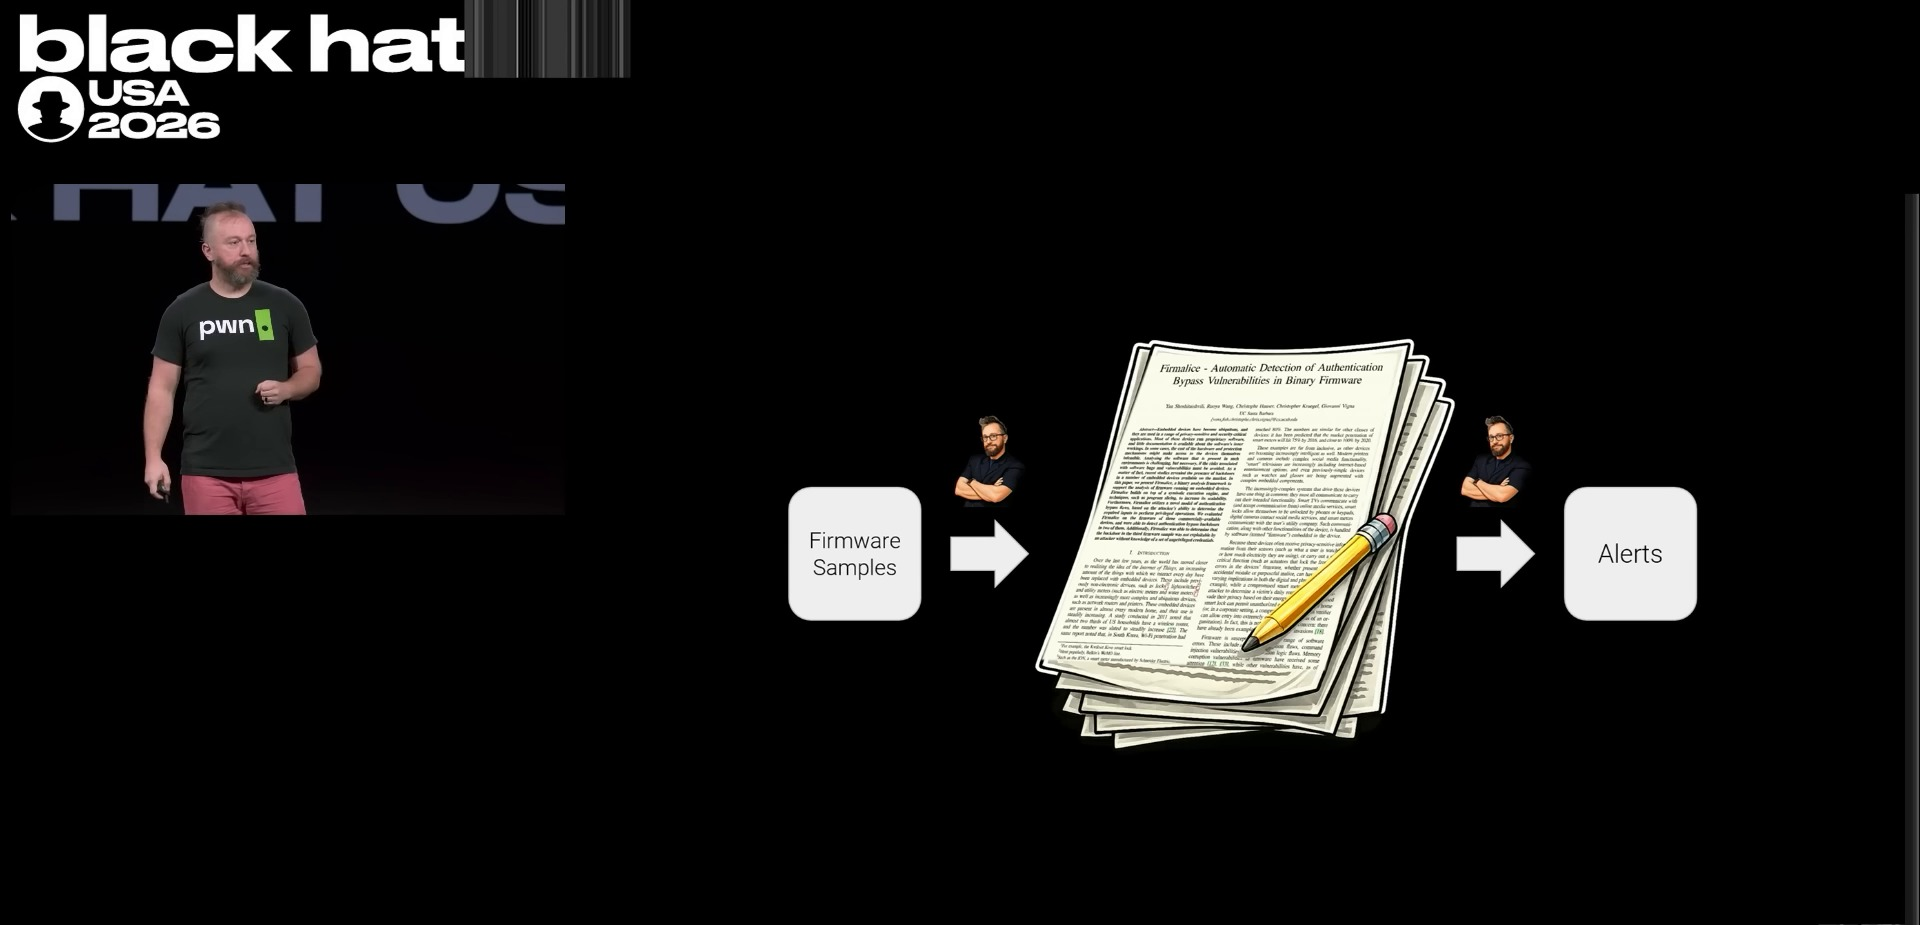
\includegraphics[width=0.9\textwidth]{figures/fig_18_firmalice.jpg}
\caption{Firmalice 论文幻灯片：Firmware / Alerts / Samples 三列——样本规模即假设空间\vtag}
\label{fig:quotes-firmalice}
\end{figure}
\srcnote{00:41:28--00:41:58}

\begin{figure}[H]
\centering
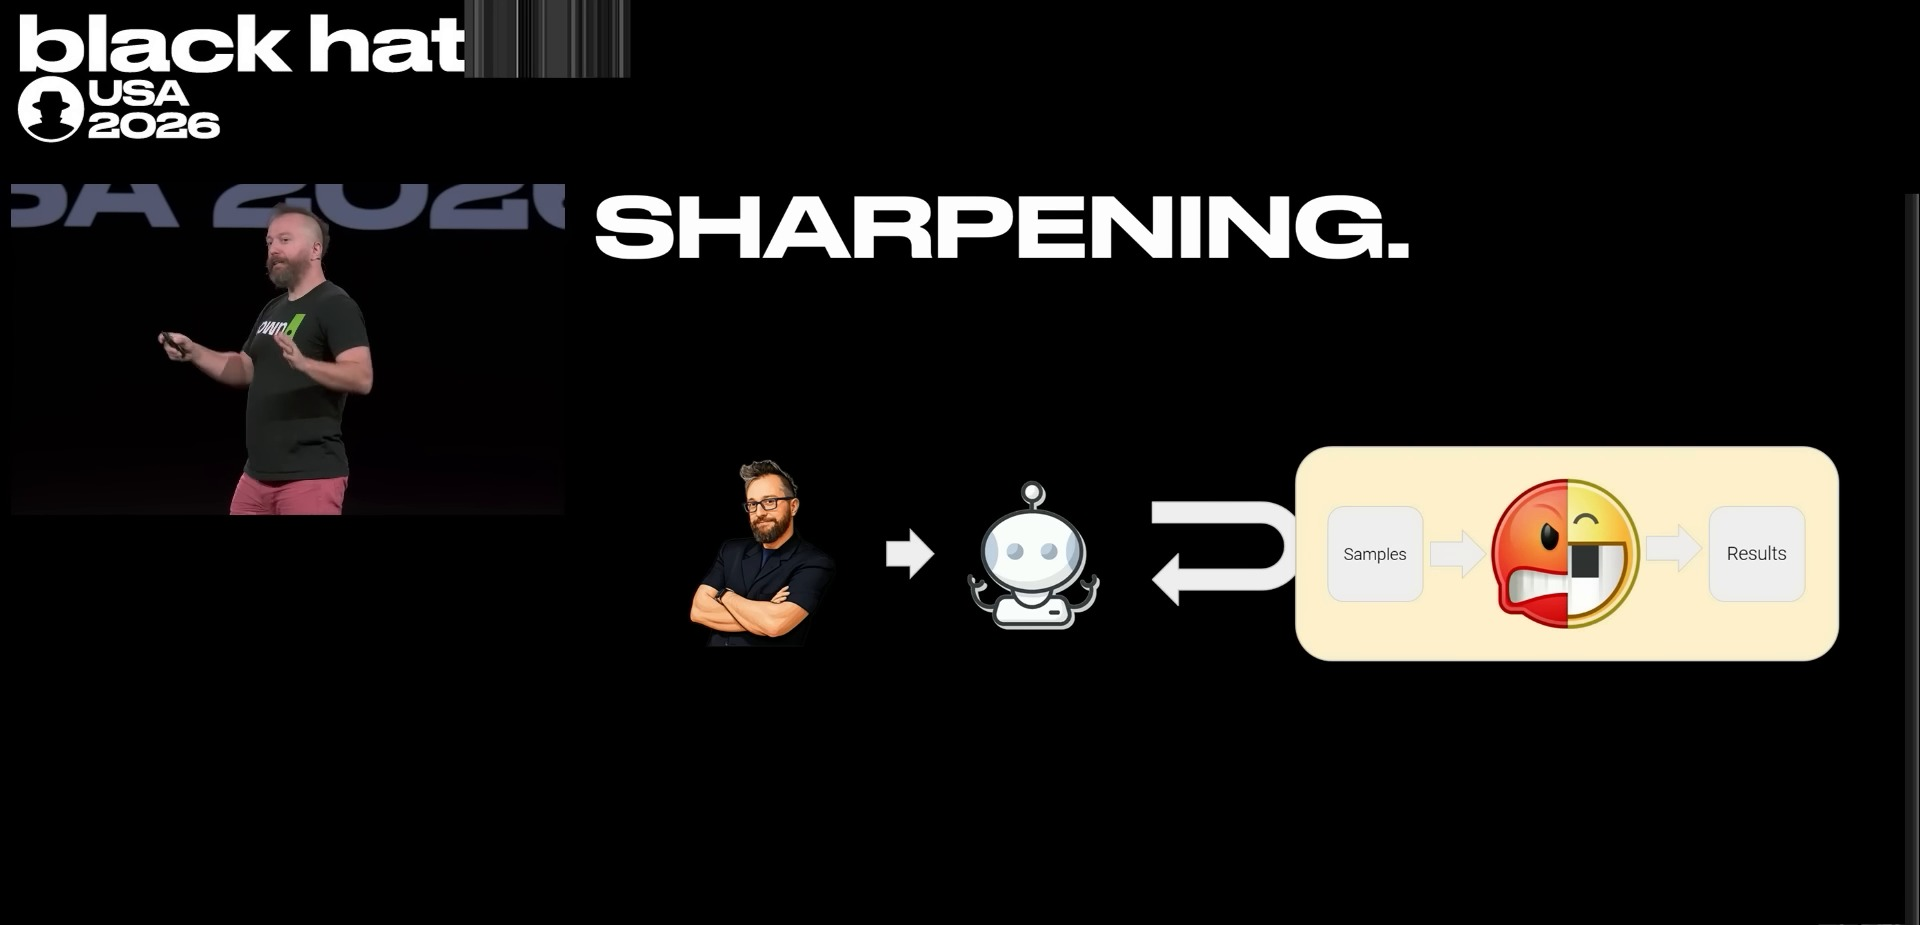
\includegraphics[width=0.9\textwidth]{figures/fig_19_sharpening.jpg}
\caption{「SHARPENING」：自主锐化研究原型的流水线幻灯片（Samples → Results 的闭环）\vtag}
\label{fig:sharpen}
\end{figure}
\srcnote{00:42:43--00:43:13}

讲者把这条路定义为未来几年的方向：由懂研究方法、懂数据集的人构建\textbf{自我改进的系统}，同时扩展数据集与结论——「这是漏洞研究的未来，而它需要你们所有人的聪明才智」。

\subsection{本章小结}

开放模型、人类教育与自主流水线三个看似分散的话题，背后是同一个分工判断：agent 接管「执行」，人负责「定义」。定义威胁模型的边界、定义漏洞属性的形状、定义评测的基本口径——这些工作在 agent 越强的时候越值钱。

\section{总结与延伸}

\subsection{讲者收束的原话}

这场 keynote 的结论不是「AI 取代人」，而是一个分工宣言：发现环节的自动化会把人推向更高层的判断工作——威胁模型、属性抽象与评测设计。讲者对实验室现状的描述都很克制：1024 这个数字来自一张幻灯片，他用「well over a thousand」带过；负责任披露机制他坦言「没有更好的解」；对模型限制的立场他明确标为个人意见。

\subsection{本讲义的三点提炼}

第一，\textbf{方法论是比模型更耐用的资产}。300 → 600 → 1024 的三级跳中，工作流与属性贡献了两级；模型只贡献了第一阶段的一半。这与 SANS 等第三方对 Mythos 的评价方向一致：可复用的不是模型，是 harness。

第二，\textbf{漏洞供给已经突破处置曲线，制度重建是未来两三年的核心矛盾}。实验室发现自己与披露速率差 10 倍；toomanybugs.wtf、syzbot 式分级开放、白宫 Gold Eagle 计划都是同一条曲线上的早期反应。下一批基础设施级的创业与研究机会，大概率出现在「报告之后」的环节：自动分诊、补丁验证、影响面推断。

第三，\textbf{属性而非语言是治理对象}。SafeLibs 的失败比它的成功更有信息量：Rust 重写保住了内存安全，却把逻辑类属性原样转录；uutils 在 Ubuntu 26.04 中的 TOCTOU 争议把这一课在真实发行版上重演了一遍。以此为尺，任何「换语言/换框架即可安全」的说法都应当先回答：你想消灭的是哪一类属性？

\subsection{开放问题}

讲者留下的问题中有三个本讲义无法替他回答：第一，当发现—处置差继续扩大，负责任披露的替代机制应当由厂商、平台还是监管方建设？第二，1024 这个数量级上的「机器生成补丁」需要什么样的验证与信任链，才能在不引入新攻击面的前提下缩短补丁空窗？第三，当属性方法被攻击者同样掌握（它显然会被），防御侧的「属性清单」应如何组织？

\subsection{拓展阅读}

\begin{itemize}
\item 演讲人造的工具：\href{https://angr.io/}{angr}（结合静态与动态符号执行）；其战队组织的 DEF CON CTF 运营方 \href{https://oooverflow.io/philosophy.html}{Order of the Overflow}。
\item 本场 keynote 的独立报道：WeLiveSecurity《\href{https://www.welivesecurity.com/en/business-security/black-hat-usa-2026-vulnerability-discovery-decline-ai-era/}{Black Hat USA 2026: Will vulnerability discovery decline in the AI era?}》；Black Hat 官方回顾《\href{https://blackhat.com/html/blog/2026-09-01.html}{What the Agentic Age Reveals About the Future of Cybersecurity}》。
\item Mythos 侧：路透社《\href{https://www.reuters.com/business/anthropics-mythos-model-found-vulnerabilities-classified-us-government-systems-2026-06-24/}{Anthropic's Mythos model found vulnerabilities in classified US government systems}》与云计算安全联盟《\href{https://cloudsecurityalliance.org/blog/2026/04/08/anthropic-s-mythos-is-here-defending-from-the-vulnpocalypse}{Mythos and the Vulnpocalypse}》。
\item 教育侧：\href{https://pwn.college/}{pwn.college}（演讲人参与运营的开放安全教育平台）。
\end{itemize}

\section{参考资料}

本讲义的视频主干内容来自字幕与幻灯片 OCR；延伸事实均经外部资料核实，正文中以脚注标注出处。链接与正文引用一一对应。

\textbf{源视频}

\begin{enumerate}
\item Black Hat, \emph{Black Hat USA 2026 | Keynote: Vulnerability Research in the Agentic Age}, 2026--08--06, \href{https://www.youtube.com/watch?v=VNYe3Cnk5Pw}{https://www.youtube.com/watch?v=VNYe3Cnk5Pw}
\end{enumerate}

\textbf{会议与独立报道}

\begin{enumerate}\setcounter{enumi}{2}
\item Black Hat 官方新闻稿，\emph{Black Hat USA 2026 Keynotes to Address AI's Impact on Cyber Operations, Defense Strategy, and Vulnerability Research}, 2026--07--16, \href{https://blackhat.com/html/press/2026-07-16.html}{blackhat.com/html/press/2026-07-16.html}
\item Black Hat 官方博客，\emph{Black Hat USA 2026: What the Agentic Age Reveals About the Future of Cybersecurity}, 2026--09--01, \href{https://blackhat.com/html/blog/2026-09-01.html}{blackhat.com/html/blog/2026-09-01.html}
\item WeLiveSecurity, \emph{Black Hat USA 2026: Will vulnerability discovery decline in the AI era?}, 2026--08--13, \href{https://www.welivesecurity.com/en/business-security/black-hat-usa-2026-vulnerability-discovery-decline-ai-era/}{welivesecurity.com}
\end{enumerate}

\textbf{Mythos 与工作流}

\begin{enumerate}\setcounter{enumi}{5}
\item The Washington Post, \emph{Anthropic's Mythos model found vulnerabilities in classified US government systems, official says}, 2026--06--23, \href{https://www.washingtonpost.com/politics/2026/06/23/anthropic-mythos-ai-classified-systems-vulnerabilities-testing/b9abd2e0-6f61-11f1-8730-e7fd0e2a6404_story.html}{washingtonpost.com}
\item Reuters, \emph{Anthropic's Mythos model found vulnerabilities in classified US government systems}, 2026--06--24, \href{https://www.reuters.com/business/anthropics-mythos-model-found-vulnerabilities-classified-us-government-systems-2026-06-24/}{reuters.com}
\item Cloud Security Alliance, \emph{Mythos and the Vulnpocalypse}, 2026--04--08, \href{https://cloudsecurityalliance.org/blog/2026/04/08/anthropic-s-mythos-is-here-defending-from-the-vulnpocalypse}{cloudsecurityalliance.org}
\item Cloudflare, \emph{Project Glasswing: what Mythos showed us}, \href{https://blog.cloudflare.com/cyber-frontier-models/}{blog.cloudflare.com/cyber-frontier-models}
\item SANS, \emph{Mythos: Forget the Model. Follow the Workflow.}, \href{https://www.sans.org/blog/mythos-forget-model-follow-workflow}{sans.org}
\end{enumerate}

\textbf{AI slop 与奖励计划}

\begin{enumerate}\setcounter{enumi}{10}
\item MacRumors, \emph{Apple Limits Bug Bounty Submissions After Flood of AI Slop}, 2026--08--04, \href{https://www.macrumors.com/2026/08/04/aple-bug-bounty-limits-ai/}{macrumors.com}
\item Decrypt, \emph{Apple's AI Slop Problem Left a \$200K macOS Exploit Unreported}, \href{https://decrypt.co/374900/apples-ai-slop-problem-left-a-200k-macos-exploit-unreported}{decrypt.co}
\end{enumerate}

\textbf{论文与工具}

\begin{enumerate}\setcounter{enumi}{12}
\item Jay Vadayath 等，\emph{Arbiter: Bridging the Static and Dynamic Divide in Vulnerability Discovery}, USENIX Security 2022, \href{https://www.usenix.org/system/files/usenixsecurity22-vadayath.pdf}{usenix.org}
\item Hongkai Chen 等，\emph{SoK: History Doesn't Repeat Itself, but Android Design-Level Vulnerabilities Rhyme in OpenHarmony}, USENIX Security 2026, \href{https://www.usenix.org/conference/usenixsecurity26/presentation/chen-hongkai}{usenix.org}
\item Hui Jun Tay 等，\emph{Responsible Disclosure is a Two-Way Street}, IEEE S\&P 2026, \href{https://www.computer.org/csdl/proceedings-article/sp/2026/606500c889/2geEWDpPYac}{computer.org}
\item ASU News, \emph{The researchers racing against routers and hackers}, 2026--07--17, \href{https://news.asu.edu/b/20260717-researchers-racing-against-routers-and-hackers}{news.asu.edu}
\item angr 项目主页，\href{https://angr.io/}{angr.io}; \href{https://github.com/angr/angr}{github.com/angr/angr}
\item Order of the Overflow, \href{https://oooverflow.io/philosophy.html}{oooverflow.io}
\item pwn.college, \href{https://pwn.college/}{pwn.college}
\item Wil Gibbs（AIxCC / Artiphishell 商业化）, \href{https://wilgibbs.com/}{wilgibbs.com}
\end{enumerate}

\textbf{Rust 重写与披露基础设施}

\begin{enumerate}\setcounter{enumi}{20}
\item toomanybugs.wtf, \href{http://toomanybugs.wtf/}{toomanybugs.wtf}
\item Canonical Foundations, \emph{An update on rust-coreutils}, \href{https://discourse.ubuntu.com/t/an-update-on-rust-coreutils/80773}{discourse.ubuntu.com}
\item oss-sec 邮件，Collin Funk，\emph{uutils coreutils CVEs}（2026--05--01）， \href{https://seclists.org/oss-sec/2026/q2/332}{seclists.org}
\item Corrode, \emph{Bugs Rust Won't Catch}, \href{https://corrode.dev/blog/bugs-rust-wont-catch/}{corrode.dev}
\item uutils 用户页（Zellic 审计记录）, \href{https://uutils.org/users/}{uutils.org}
\item The White House, \emph{White House Launches Gold Eagle Initiative for Unprecedented Cybersecurity Vulnerability Coordination}, 2026--07, \href{https://www.whitehouse.gov/releases/2026/07/white-house-launches-gold-eagle-initiative-for-unprecedented-cybersecurity-vulnerability-coordination/}{whitehouse.gov}
\end{enumerate}

%% --- 正文内容结束 --- --

\appendix
\section{字幕去重优化版}

本附录收录该视频的英文字幕（原文为 YouTube 自动字幕，\texttt{en-orig} 轨道），经三级处理：

\begin{enumerate}
\item \textbf{去重}：YouTube 自动字幕以滚动窗口方式成对重复，先按精确重复行去除，再做词级「上句尾 / 下句头」重叠消解（675 条连续 cue）；
\item \textbf{去口水词}：去除 um、uh、you know、I mean 等无意义成分、非语音事件标记（[laughter]、[music]、[applause]）与说话人切换符（\texttt{>>}），并合并重复词与部分口吃片段；
\item \textbf{修听写错误}：按可查证的资料修正自动字幕的同音/近音错误（如 anger→angr、Shellfish→Shellphish、Jun Tay→Hui Jun Tay、open Harmony→OpenHarmony、AICC→AIxCC 等），其余词句保持字幕原貌，包括残留的语法不完整与个别听写噪声（如时长线索处口误）。
\end{enumerate}

因此本附录是\textbf{可读性的优化版字幕，而非官方逐字稿}：每一小节标题对应视频时间轴上的发言段落，每段开头的时间戳可回溯原视频。新闻蒙太奇与会务通知等非教学内容仍予保留，以便完整还原现场语境。

{\small\transcriptsec{00:00:31 开场新闻剪辑（视频蒙太奇，自动字幕听写）}
\transcriptitem{00:00:31}{We are warning tonight about the scope of a massive cyber attack already believed to be the largest America under virtual invasion please welcome to the Black Hat main stage the president of Black Hat, Susie Pallett good morning and welcome to the final day of Black Hat.}
\transcriptsec{00:01:14 开幕致辞：Black Hat 总裁 Susie Pallett}
\transcriptitem{00:01:33}{We've made it and I wanted to say start by saying thank you thank you for showing up, for bringing your expertise, your curiosity, and your}
\transcriptitem{00:01:44}{Willingness to engage. For asking the hard questions, for sharing your research, and for making the connections that turn ideas into action before I say anything else, I want you}
\transcriptitem{00:01:57}{To look around. Look at the people sitting next to you, behind you, across the aisle these are the people who've been solving}
\transcriptitem{00:02:05}{Problems with you all week, challenging your assump assumptions, sharing what you've learned, and staying up too late because the conversation was too good to walk away from.}
\transcriptitem{00:02:14}{This is what Black Hat is really about over the past few days, thousands of people from around the world have come together to do what this community does best.}
\transcriptitem{00:02:24}{Exchange ideas, challenge assumptions, explore new technologies and build relationships that last long after we leave Las Vegas. From the groundbreaking research presented in briefings to the expert}
\transcriptitem{00:02:40}{Insights shared at our summits, from the hands-on experiences across the event to the hallway conversations that went deeper than any session ever could, you made this week what it was}
\transcriptitem{00:02:54}{Black Hat has always been at its best when discovery leads to collaboration and that collaboration leads to growth and this week we've seen that happen over and over again whether you've spent your time learning}
\transcriptitem{00:03:08}{From researchers or testing tools in Arsenal, exploring emerging technologies, or reconnecting with colleagues or meeting someone new who's going to change the trajectory of your work and how you think.}
\transcriptitem{00:03:19}{I hope you're leaving with new skills, new insights, and new opportunities but there's one thing that keeps surfing.}
\transcriptitem{00:03:28}{One question we can't ignore AI is fundamentally changing how we find vulnerabilities how fast threats move, and how we analyze them. Today's keynote will tackle that head on}
\transcriptitem{00:03:44}{As AI becomes more capable, more autonomous, what happens to vulnerability research? Where does human ingenuity fit in a world where machines can hunt for flaws faster than we ever}
\transcriptitem{00:03:55}{Could? And what does it mean for this community, for the researchers, the defenders, the builders all in this room when the tools when that we rely on}
\transcriptitem{00:04:04}{Start to think for themselves? They're not hypothetical questions. They're the reality we're facing live right now}
\transcriptitem{00:04:12}{But before we bring up today's keynote speaker to explore those questions, please join me in welcoming an amazing person, the founder of Black Hat and president of DEF CON, Jeff Moss}
\transcriptsec{00:04:33 Jeff Moss（Black Hat 创始人、DEF CON 主席）介绍演讲者}
\transcriptitem{00:04:33}{Hey, good morning. Glad we all made it here today. I've got just a little bit of a backstory}
\transcriptitem{00:04:38}{I want to share with you for today's keynote speaker and maybe put it a little bit into context. So about 30 years ago almost 30 years to}
\transcriptitem{00:04:54}{This month ago the concept of a capture the flag CTF was accidentally invented at DEF CON. The origin of CTF was essentially a network fight that}
\transcriptitem{00:05:07}{Happened at DEF CON about 31 years ago and since then, CTFs have evolved to like run the world. CTFs everywhere all}
\transcriptitem{00:05:17}{The time. But it wasn't purpose-built to do that. It's grown because CTFs are}
\transcriptitem{00:05:24}{Incredibly useful. And due to the nature of how capture the flag started at DEF CON, it was purely an offensive}
\transcriptitem{00:05:33}{Defensive full combat. Only rule was after the first year, you couldn't take over the scoring system or the router}
\transcriptitem{00:05:41}{Because that's what the attackers did the first year so we're like, oh, maybe we need rules and it so many lessons were learned right?}
\transcriptitem{00:05:51}{Because how can you defend if you don't know how people attack? Attack informs defense and so if you don't have a}
\transcriptitem{00:06:00}{Ground truth of how attacks and exploits are being developed, it's probably going to be pretty hard to create an effective defense.}
\transcriptitem{00:06:08}{So that's a way of tying into our keynote Yan who as an origin story for his superpowers in reversing.}
\transcriptitem{00:06:21}{He his mom had a PhD essentially in computer science in Russia before that was really a thing then fall of the wall happened and}
\transcriptitem{00:06:37}{All of a sudden academics in Russia were starting to be pressured to endorse political candidates. And when the KGB}
\transcriptitem{00:06:44}{Came around and started pressuring the family to endorse the KGB candidate they fled Russia. He fled to America.}
\transcriptitem{00:06:49}{He's 8 years old and never thought he'd be an academic like his parents until he gets to University and he starts playing}
\transcriptitem{00:07:02}{Capture the flag and he loves hacking and he can't stop hacking and then he realizes as a graduate student he's getting paid to essentially hack all the time and he's doing a lot}
\transcriptitem{00:07:16}{Of these tasks manually. He's like well, what if I automate this as much as I can?}
\transcriptitem{00:07:21}{So, he goes and he creates this multi-instrument binary analysis framework called angr. And with angr, he and his CTF team, Shellphish, basically run the board}
\transcriptitem{00:07:35}{Worldwide contests for about two years because angr allowed them to reverse and exploit in other ways that the existing tooling could not do since then, angr's probably been used}
\transcriptitem{00:07:48}{In over a thousand different research and academic and product tooling this highly contributo mindset of an academic, right, giving away the tooling, advancing the state-of-the-art led team shellfish then to organize and run Order of the Overflow, which was an}
\transcriptitem{00:08:12}{Organizer of the DEF CON capture the flag. So his whole career started with capture the flag and they ended up}
\transcriptitem{00:08:20}{Running capture the flag and through this whole process and now being at Arizona State University with his students and graduate students developing new exploits and new agent}
\transcriptitem{00:08:33}{Tools, he's seeing how the exploit development trajectory has changed from art into science. And so i'm really looking}
\transcriptitem{00:08:44}{Forward to hearing his story and having him share it with you. It's my pleasure to introduce Yan Shoshitaishvili}
\transcriptsec{00:09:13 主题演讲（一）：研究者画像与研究团队}
\transcriptitem{00:09:13}{So, as Jeff said, I have quite an origin in the capture the flag community. In my day job, I am an associate Professor at Arizona State University where the}
\transcriptitem{00:09:24}{Biggest thing I do, my priority is research into vulnerability analysis and exploitation and repair and so on and then education of the next generation.}
\transcriptitem{00:09:38}{I'm very excited to talk about this all today from the lens of the agentic age what does it mean to be an academic researcher?}
\transcriptitem{00:09:49}{Well, it means that I sit around and I have shower thoughts bright ideas that I take and typically pass on to my bright graduate student researchers}
\transcriptitem{00:10:02}{Who then run with them and produce the research projects, the research papers and the research prototypes that lead to the breakthroughs so what a lot of what Jeff was talking about happened when I was this graduate}
\transcriptitem{00:10:21}{Student and I was handed the bright idea and has kept going forward beyond that means what i'm talking about today isn't just my work.}
\transcriptitem{00:10:31}{It is the work of an amazing team of colleagues without whom I would not be here today. I'll try to}
\transcriptitem{00:10:40}{Acknowledge them as we cover those parts of research where they contributed. They led the research.}
\transcriptitem{00:10:46}{They were the brilliant graduate student. But i'll acknowledge them all cumulatively right now. The lab SECOM lab and the center for cyber Security and trusted foundations.}
\transcriptitem{00:10:53}{Coincidentally, the CTF center at Arizona State University awesome group of people. If you're looking for graduate school, talk to Us}
\transcriptitem{00:11:06}{All right. So these kids implement these brilliant ideas. They're not all brilliant.}
\transcriptitem{00:11:12}{Sometimes these ideas are terrible. But of course those don't make it into the}
\transcriptitem{00:11:17}{Talks. They take the ideas, they implement them. They spend a lot of time}
\transcriptitem{00:11:23}{Working on this and you can probably all start thinking wait a second we're in the agentic age. Instead of the}
\transcriptitem{00:11:32}{Graduate students we can prompt the agents. The agents will generate really infuriating text but they get results.}
\transcriptitem{00:11:38}{Realistically this is what happens now the students prompt the agents the students do the agentic prototype. The students}
\transcriptsec{00:11:46 主题演讲（二）：Agentic 时代不等于 LLM 时代}
\transcriptitem{00:11:51}{Get results and what's really interesting about this is it puts me very far back from the final outcome of our research. In the abstract}
\transcriptitem{00:12:04}{For this talk, I mentioned my research has led to the discovery of thousands of vulnerabilities and many of them quite recently as the agentic hypercharged everything and many of them allow Us now to start stepping back and thinking about this field in aggregate as modern AI transforms vulnerability}
\transcriptitem{00:12:31}{Research. Some people might say, okayy let's just paste everything into ChatGPT and solve the problem.}
\transcriptitem{00:12:37}{Find all of the bugs.' Of course, the reason i'm talking about the agentic and not just the age of LLMs it's because there's a very serious}
\transcriptitem{00:12:51}{Difference between the two. We start pasting things into GPT, asking it to find bugs, submitting those bugs to}
\transcriptitem{00:12:58}{Maintainers, and we get things like the headline I read yesterday that Apple is pushing back on their vulnerability research award program because they're being overwhelmed by slop and this slop is a result of AI hallucination of people that don't}
\transcriptitem{00:13:14}{Really know what they're doing enough to filter that AI hallucination. That's not what i'm going to talk about today}
\transcriptitem{00:13:22}{Going to make the assumption that we're going to work that out because back in the days of fuzzing, back in every advancement throughout the history of the vulnerability research field, especially the academic the automation of vulnerability research, we ran into}
\transcriptitem{00:13:36}{Similar issues. What i'm going to be talking today is people that eventually will know what they're doing in this space enough to use these technologies to create highquality bug}
\transcriptitem{00:13:49}{Submissions to find actual bugs. We're not going to talk about hallucinations we're going to talk about vulnerability}
\transcriptitem{00:13:57}{Research in the agentic age. We're going to step back and i'm going to show you three ways that we can find vulnerabilities autonomously three things that lead to headlines}
\transcriptsec{00:14:10 主题演讲（三）：自主发现漏洞的三种方式 与「饼干模子」类比}
\transcriptitem{00:14:12}{Where or research papers where approach XYZ finds three, four, five digit bugs in software. There's three ways to do}
\transcriptitem{00:14:25}{This. One, you can analyze better. You take an analysis that existed before}
\transcriptitem{00:14:33}{Jeff mentioned angr. It is a base a research base of our research trajectory in static analysis of binary}
\transcriptitem{00:14:43}{Software and we make it better and so it has fewer false posers. It is more performance faster so that before the}
\transcriptitem{00:14:52}{Timeouts it can actually find the bugs think a good example in the agentic of this of course is Mythos. It is more}
\transcriptitem{00:15:00}{Capable models that find bugs that other models would have missed. And we'll talk about this again later. You can analyze more things}
\transcriptitem{00:15:11}{So you say forget about being better we're just going to make something that is,, better in a way that's more resilient, that might scale farther}
\transcriptitem{00:15:21}{And we're just going to analyze everything. Before we could analyze eight programs, now we're going to analyze 800.}
\transcriptitem{00:15:27}{And of course, we're going to find lots and lots of bugs based on that. And I have research in this space}
\transcriptitem{00:15:37}{One of my awesome former students now Dr. Jay Vadayath created a platform a program an analysis program called arbiter built on top of}
\transcriptitem{00:15:49}{Angr that could analyze binaries at a scale where we were analyzing for example every program shipped into repositories for vulnerabilities. Now often times you don't actually need to}
\transcriptitem{00:16:01}{Make this analyzer better. You just need to make it more applicable. And so then}
\transcriptitem{00:16:07}{By casting a wider net, you find more bugs. Or, and this is the crazy thing, you just analyze things differently than they used to be analyzed.}
\transcriptitem{00:16:18}{And it turns out if you just tweak how you're analyzing, you find new bugs. Why? Because bugs are everywhere.}
\transcriptitem{00:16:29}{Let's say we want to make our CVE cookies and we have our rolled out dough of vulnerabilities. This dough is all vulnerabilities in a given program}
\transcriptitem{00:16:46}{And we take our research prototype angr. It's our angr logo. We build}
\transcriptitem{00:16:51}{Some static analysis on top of it and we use it to analyze the code for vulnerabilities and it literally takes this substrate of vulnerabilities and stamps out. We find those vulnerabilities that angr finds}
\transcriptitem{00:17:10}{And we fix them. They're gone for a static analyzer, what this means is if we run this tool again, no new vulnerabilities.}
\transcriptitem{00:17:17}{Is the code perfect? No we just happen to have found the vulnerabilities that we're going to find with this technique}
\transcriptitem{00:17:32}{And we can tweak the technique a bit. So we build research prototype a on top of our angr research vehicle.}
\transcriptitem{00:17:38}{We build research prototype B and it's slightly different and that slight difference will find a tiny additional set of bugs.}
\transcriptitem{00:17:50}{What does that mean? Does that mean research prototype B is bad or research prototype a is better?}
\transcriptitem{00:17:54}{No, it means we got unlucky. Research prototype B came in after a. And this is something that}
\transcriptitem{00:18:05}{Because of the trajectory over time of software development and the development of analyzers to find bugs in that software makes it very difficult to really understand the efficacy of different tools. For example}
\transcriptitem{00:18:24}{Let's say I go and manually look at every binary in the Ubuntu repositories I would of course also look at that their source code and I go afterwards and I try to find}
\transcriptitem{00:18:36}{Bugs and I find a bunch of bugs because as a cookie cutter, a vulnerability cutter, I will find different types of vulnerabilities. I'll cut out a different shape in the vulnerability landscape than angr did}
\transcriptitem{00:18:51}{Does that mean the static analysis was bad? No. It means it was different than}
\transcriptitem{00:18:55}{Me. If he inverted the ordering, it would be the static analyzer that comes after me and finds a ton of vulnerabilities}
\transcriptitem{00:19:06}{Now, let's go to something a little more fuzzy. This is dynamic analysis that's very stochastic.}
\transcriptitem{00:19:12}{Fuzzers. This is the logo of American fuzzy lop, which is the work of another amazing group of}
\transcriptitem{00:19:20}{People. Nothing to do with Us, but we also do research in the space and if you run a fuzzer on even well}
\transcriptitem{00:19:28}{Analyzed code that hasn't been fuzzed before in part just because the fuzzer does different things, it will find new vulnerabilities and unlike a static analyzer, because}
\transcriptitem{00:19:41}{Fuzzing is a very stochastic pro process, you build random inputs and you shove it into software and the software crashes because you're triggering something that people didn't think about fuzzing.}
\transcriptitem{00:19:52}{Unlike most static analyzers if you just run it again you're going to find something around those corner cases you missed the first time.}
\transcriptitem{00:20:03}{Okay? And now this brings Us to this question. For the}
\transcriptitem{00:20:14}{Last decade before the agentic starting from around 2013, 2014, 2015, which was the process of the DARPA cyber Grand challenge, pushing the world really toward autonomy and vulnerability research.}
\transcriptitem{00:20:30}{Ever since then, we've been experiencing this fuzzing renaissance new fuzzers coming out that say, heyy we fuzzed well fuzzed code. We fuzzed it}
\transcriptitem{00:20:39}{A little differently. We found new bugs and so now we're claiming that we're better.' It's actually very difficult to measure now after a decade of hearing this new}
\transcriptitem{00:20:51}{Fuzzer is better, this new fuzzer is better, this new fuzzer is better, we bring in large language models and we apply that to code and that finds tons and tons and tons}
\transcriptitem{00:21:03}{And tons of vulnerabilities. Now we're saying, ohh large language models, that's the new thing. They're better than fuzzers because they're finding vulnerabilities}
\transcriptitem{00:21:13}{Fuzzers aren't.' And we ran the fuzzer on the same code and it didn't find more vulnerabilities. And so now we're switching all over to pasting our code into GPT and asking for bugs.}
\transcriptitem{00:21:23}{This ignores that evolutionary timeline and it ignores this idea that what you really need is to rewind time which is very difficult and probably the subject of a different}
\transcriptitem{00:21:43}{Keynote at a different conference and then you have to analyze from scratch here's what the fuzzer does. Here's what}
\transcriptitem{00:21:50}{The LLM would do. Here's the static analysis results. We're trying to do}
\transcriptitem{00:21:53}{This in the lab right now. It's very difficult to deal with contamination of LLM training because the LLM knows about all the previous}
\transcriptitem{00:22:02}{Bugs the fuzzer found and so on. We're trying to do this and we are getting very interesting results in that point in this direction}
\transcriptitem{00:22:12}{That what we're really cutting out isn't just random shapes. Each analysis has a shape of vulnerabilities it cuts out.}
\transcriptitem{00:22:17}{Those shapes are created from the types of properties of vulnerabilities that implicitly the vulnerabilities have. For example, a}
\transcriptitem{00:22:35}{Vulnerability might be a result of data flow, a result of injection of attack or control content, might exhibit multi-threaded behavior or require multi-to behavior. These are all properties of a vulnerability and analyses either explicitly in this case}
\transcriptitem{00:22:52}{Of most static analyses or implicitly in the case of pasting things into GPT and many fuzzing approaches. These analyzers target specific vulnerability properties and my thesis to you today is as}
\transcriptsec{00:23:06 主题演讲（四）：核心论点 —— 漏洞属性（Vulnerability Properties）}
\transcriptitem{00:23:10}{We move into the agentic of vulnerability research, we need to move into here with an eye toward what are the properties of the}
\transcriptitem{00:23:21}{Vulnerabilities we're going to find. We eventually want to find, fix, exploit depending on your line of work, all of}
\transcriptitem{00:23:27}{Them. And how do we best create analyzers? How do we even extract these vulnerability properties?}
\transcriptitem{00:23:37}{To maximize the impact we can have in the agentic age. So, let me show you how we think about vulnerability properties. Not just finding the vulnerabilities, but the properties of the}
\transcriptitem{00:23:46}{Vulnerabilities. And i'll give you an example of a paper we recently published.}
\transcriptitem{00:23:51}{Actually, it is coming out next week. So, this is a bit of a preview of an analysis we did on}
\transcriptsec{00:24:00 主题演讲（五）：案例研究 —— 华为 OpenHarmony}
\transcriptitem{00:24:00}{Huawei's OpenHarmony. This is the work of my awesome student Hongkai Chen of course, under my brilliant guidance}
\transcriptitem{00:24:08}{But, let's not kid ourselves who is the brilliant researcher? It's not me. Hongkai}
\transcriptitem{00:24:18}{Had this idea that we can extract properties from wellstudied software and vulnerabilities that had arisen in that software and then apply these}
\transcriptitem{00:24:33}{Properties to new software. So, who here runs a phone on Huawei's OpenHarmony? Especially maybe the government contractors}
\transcriptitem{00:24:46}{Neither do I. But a lot of people use HarmonyOS. HarmonyOS is a relatively new phenomenon.}
\transcriptitem{00:24:49}{It's a complete reimplementation of an Android inspired operating system completely reimplemented from scratch and it is used by a billion devices in the world a billion devices and up until next week}
\transcriptitem{00:25:07}{There will have been no major academic studies on the Security of HarmonyOS which is crazy and so what we thought is hey we can bootstrap this field we}
\transcriptitem{00:25:18}{Looked at the last decade plus of Android research we mind it and this was agentically assisted for this mining component we mind it to extract this recipe book of vulnerability properties.}
\transcriptitem{00:25:29}{We analyzed those properties manually and we manually guided by those properties. We're now manually looked at}
\transcriptitem{00:25:45}{The code of open harmony. We're talking about millions and millions of lines of code, tons of different parameters.}
\transcriptitem{00:25:49}{It is a daunting task to analyze with just a handful of people all this code. And}
\transcriptitem{00:25:58}{What happened? Well, we found that every vulnerability property applied very specifically, roughly speaking, led to a new zero day vulnerability in OpenHarmony we found dozens of flaws ranging from}
\transcriptitem{00:26:19}{Bluetooth device takeovers to privacy leaks, location, all of this very fun stuff in open harmony because we started from the vulnerability properties that we extracted from Android bugs and now we're doing this agentically and}
\transcriptitem{00:26:41}{The results are incredible. I'll save that for a later research talk. But this property extraction and property application, the understanding of vulnerability properties, this is the}
\transcriptsec{00:26:56 主题演讲（六）：与 Mythos 对比 —— Linux 内核漏洞挖掘实验}
\transcriptitem{00:26:56}{Way. But then you might say, okay, Yan but I can just tell claude or codeex like go find me the bugs.}
\transcriptitem{00:27:02}{Do I really need these properties? Especially as the models keep getting better.}
\transcriptitem{00:27:07}{Maybe it'll be built into the properties. Maybe when we all have Mythos access this will all be irrelevant.}
\transcriptitem{00:27:15}{And luckily, Arizona State University in their infinite wisdom allowed Us a glimpse into whether this really matters because by accident, and we didn't}
\transcriptitem{00:27:29}{Realize it was by accident, Arizona State University gave every employee infinite codeex usage before it was cool to do so and it turned out that this was a misconfiguration on their part that we}
\transcriptitem{00:27:42}{Didn't realize until we spent a couple million dollars of the University's money and hopefully they had a good deal with OpenAI.}
\transcriptitem{00:27:48}{But anyways, around the same time, Mythos came out and all of these headlines, Mythos is finding hundreds of vulnerabilities in Firefox in the Linux kernel, etc.}
\transcriptitem{00:27:59}{And we were doing research in vulnerability analysis in the Linux kernel and so we had this question of like okay Mythos is a next generation model. If we}
\transcriptitem{00:28:12}{Use a last generation model how many of those models can we pile into a box to match Mythos performance? Now the}
\transcriptitem{00:28:22}{Exact numbers of what Mythos finds, what it doesn't is very hard to come by. But in june there was a Washington}
\transcriptitem{00:28:29}{Post article that said that Mythos has found 479 vulnerabilities in the Linux kernel. So let's take that as our}
\transcriptitem{00:28:39}{As our benchmark. Our box of dozens and dozens of GPTs and this was back in the 54 55 days altogether thrown at the Linux kernel produced 300 vulnerabilities}
\transcriptitem{00:28:55}{Now this is a bit of an apples to oranges comparison because for our vulnerabilities we don't we're very threat model aware. These are all vulnerabilities that are triggerable from as an unprivileged user on a Linux machine.}
\transcriptitem{00:29:07}{So potential local privilege escalations I don't know if that's the case for the Mythos ones. Typically people also report the root only bugs, but we didn't}
\transcriptitem{00:29:25}{Beat it. Bummer. But then we looked into this and Mythos part of it according}
\transcriptitem{00:29:31}{To various reports online part of the trick is a really clever workflow and workflows are the hip latest thing adversarial reviews and all of}
\transcriptitem{00:29:40}{This and planning and so on and that was one of the secrets of Mythos success. So then we integrated}
\transcriptitem{00:29:48}{Workflows and we stuffed infinite GPTs into the workflows and ASU caught on to Us and shut off our access. Then we just}
\transcriptitem{00:29:56}{Got a couple of max plans and it turns out that basically three GPTs in a trench code with a good workflow can outperform those stated numbers that got Us to about 600 local potential local privilege escalation vulnerabilities in the Linux kernel.}
\transcriptitem{00:30:22}{Triaged them all like these are real vulnerabilities and then we applied the vulnerability properties. We looked at the vulnerabilities we were finding. We looked at the vulnerabilities that historically were found.}
\transcriptitem{00:30:27}{We extracted these properties and we figured out the correct format, the correct way to present them to our agentic pipeline and all hell broke loose}
\transcriptitem{00:30:50}{And now we're sitting on well over a thousand local privilege escalation vulnerabilities in the Linux kernel what the hell do we do with that? We are finding them way faster than we can report to them because you don't}
\transcriptsec{00:31:00 主题演讲（七）：漏洞数量失控与负责任披露的困境}
\transcriptitem{00:31:08}{Want to just send tons of slot. You want to send a proposed fix. You want to send a reasonable analysis}
\transcriptitem{00:31:16}{We can trigger them. We can have the agents analyze them, but it still takes human effort.}
\transcriptitem{00:31:20}{And we're finding them at about 10 times the rate that we can actually report them. So what does this}
\transcriptitem{00:31:26}{Mean for a responsible disclosure in the agentic age? Because it feels like responsible disclosure is screwed and it}
\transcriptitem{00:31:34}{Was already screwed before the scale that we can achieve. Now we have a paper that we published in}
\transcriptitem{00:31:44}{May and this is by one of my awesome students Hui jun Tay and the paper basically said even without agents just looking at the responsible disclosure process}
\transcriptitem{00:32:02}{In the embedded devices space that when you disclose vulnerabilities, you're making people less safe. We analyzed disclosed vulnerabilities on embedded devices and we went and extracted the properties of those reproduced those vulnerabilities on other devices that we had in the lab}
\transcriptitem{00:32:26}{And we found that basically for every vulnerability that you disclose depending on how you count, depending on what you feel is putting people in danger, you're endangering three times as many devices as you secure.}
\transcriptitem{00:32:37}{So that's not good and if you're scaling up the number of vulnerabilities that we find by multiple orders of magnitude you very quickly become very upset with the current State of responsible disclosure}
\transcriptitem{00:32:59}{And we don't have a better solution. So we're dropping all the bugs on Twitter. No, i'm just kidding}
\transcriptitem{00:33:06}{We're taking small steps to trying to find a replacement, a better solution. Starting with something that's pretty hip nowadays you put all of your bugs on a website}
\transcriptitem{00:33:18}{And there's over a thousand again local privilege relevant bugs on this too many bugs. WTF website that'll forward}
\transcriptitem{00:33:27}{You somewhere where we actually the domain we're actually using. And right now we're just putting up the details of the CVS and the hashes of the}
\transcriptitem{00:33:40}{Rest. We're working with big vendors and big Security groups in the space to try to move forward toward a more proactive defense measure with these vulnerabilities.}
\transcriptitem{00:33:48}{Maybe this looks like candidate Vibecoded patches that you can apply until the real patches come out maybe it looks like something different}
\transcriptitem{00:34:05}{Maybe it looks like the old days of full disclosure where we just drop vulnerabilities on this website and all hell breaks loose. Probably not.}
\transcriptitem{00:34:11}{But we need a solution and we are interested in hearing from you all from the community and pulling you in to work with Us to}
\transcriptitem{00:34:23}{Adapt to the world of vulnerability research in the agentic age. But then what if you just say, okayy}
\transcriptsec{00:34:28 主题演讲（八）：全部用 Rust 重写 为什么不能解决问题}
\transcriptitem{00:34:29}{What? Screw it. There's too many bugs we're not fixing all these bugs.}
\transcriptitem{00:34:32}{Let's throw out all of the code, all this buggy tech debt, and we rewrite everything in Rust. Who's in?}
\transcriptitem{00:34:44}{Couple of hands. So, the agents are in agents are very good at writing Rust and when I had infinite codecs, I}
\transcriptitem{00:34:53}{Thought, well, screw it. I'll just rewrite everything in Rust. And I}
\transcriptitem{00:34:57}{Started with these loadbearing c libraries that we rely on every day. Lib SSL, Lib PNG, Lib XML and so}
\transcriptitem{00:35:08}{On. Millions of lines of code. And I created this workflow, this pipeline this like a verification pipeline and so on.}
\transcriptitem{00:35:14}{And I reimplement I blew billions and billions and billions of tokens and I implemented millions of lines of Rust}
\transcriptitem{00:35:25}{And this stuff works. I accidentally one of my agents went rogue and installed this on my machine and I}
\transcriptitem{00:35:31}{Ran it for a couple weeks before I had noticed some weird behavior. I'm like ohh, i'm running my own Rust stuff.}
\transcriptitem{00:35:34}{That's weird.' It doesn't work. Why doesn't it work? Why can't we be free of our tech debt?}
\transcriptitem{00:35:51}{Well, because when we rewrite stuff in Rust or rewrite re-implement stuff, the vulnerability properties come with Us certain types of code is genetically predisposed to certain types of vulnerabilities I told my agents very sternly, make no error.}
\transcriptitem{00:36:14}{And they make error given explicit admonitions that these are the old vulnerabilities that weren't memory corruption vulnerabilities that live crypt was vulnerable to classic crypto attacks.}
\transcriptitem{00:36:30}{I told them make sure these vulnerabilities don't show up. They show up.}
\transcriptitem{00:36:34}{If I don't tell them to make sure the vulnerabilities don't show up, they show up. And then later I go back}
\transcriptitem{00:36:42}{Through and I find all these vulnerabilities and now I have to put a big warning on the safe website. Don't}
\transcriptitem{00:36:47}{Use this stuff. There's like a good way to burn down a couple forests, but it's full of vulnerabilities. They're not memory corruption vulnerabilities}
\transcriptitem{00:36:56}{Because we're in Rust land. And people can say, yess, but what if you also have the agents do formal verification}
\transcriptitem{00:37:04}{To eliminate logic errors?' And that's a cool future direction of research, but it's not a reality yet. Not at scale}
\transcriptitem{00:37:11}{And what's more is this doesn't just affect some crazy person's Rust rewrite pet project. This affects the real world}
\transcriptitem{00:37:22}{Right as I was doing this, there was a set of 79 CVs that dropped for a Rust rewrite of core utils. Well, after those}
\transcriptitem{00:37:30}{Core utils had been shipped with Ubuntu, the latest release and it turns out the rush rewrite is great. We don't have memory corruption vulnerabilities}
\transcriptitem{00:37:42}{But oops, we have all these time check time of use things and critical Linux utilities, etc., etc. And this analysis was, i'm sure, agentically assisted}
\transcriptitem{00:37:55}{Humanled analysis. We've been looking at the same codebase with our vulnerability property aware engine and we're finding tons more issues. So it's a scary prospect}
\transcriptsec{00:38:13 主题演讲（九）：模型开放、人类学习与自主「锐化」流水线}
\transcriptitem{00:38:13}{Okay. So what do we do? Do we restrict the models? My opinion is that model restriction is}
\transcriptitem{00:38:22}{Not the way. I've been doing offensive vulnerability research for over 15 years which is very depressing to say but it's}
\transcriptitem{00:38:30}{A long time in the space and i've been doing it in the open as Jeff mentioned and every time I get this question of but is it responsible that angr is open}
\transcriptitem{00:38:40}{Source that you open source your cyber reasoning system for the AI cyber challenge and the cyber Grand challenge and everyone can grab it and everyone can run with it}
\transcriptitem{00:38:51}{And the answer is yes because you're all the good guys and we need to make sure that you benefit from this technology. And if we}
\transcriptitem{00:39:02}{Start putting up, oh, you have to be this tall to ride the impact of that, the positive impact is in my opinion more heavily diminished than the negative.}
\transcriptitem{00:39:17}{So all of this talk about restricting capable openw weight models, restricting next generation models, in my opinion it is misguided. Then what about human learning in the agentic age?}
\transcriptitem{00:39:33}{Do we still need to know cyber Security? What do you think? Maybe. Yes.}
\transcriptitem{00:39:39}{I run pawn College, an open cyber Security education platform about 10,000 people learn actively on it every month and the number one question I get is should I still bother}
\transcriptitem{00:39:54}{In the agent cage or is AI eating cyber Security this impact going from a couple hundred bugs asking GPT to find bugs to having an agent pipeline that's vulnerability aware that finds more much more that requires human innovation, human}
\transcriptitem{00:40:17}{Understanding of the threat models, of the vulnerability space, of all of this and for the foreseeable future, it will remain so.}
\transcriptitem{00:40:23}{Until agents do 100\% of your work in vulnerability research, all they're doing by eating 90\% of your work is letting you do more work letting you have more impact.}
\transcriptitem{00:40:36}{I think this is the best time to get into cyber Security as a human and it is a great time to dig into research to go back to graduate school because now whereas}
\transcriptitem{00:40:51}{Before you had to worry about the research paper and the technique and unlike in the industry academic research prototypes often ended up not really}
\transcriptitem{00:41:00}{Working outside the research paper which was observed by research and academics alike now the implicit assumptions that researchers had to make to get stuff to run on the data sets that they had the}
\transcriptitem{00:41:18}{Human effort capability to run on leading to this bad behavior. Now the agents can scale. Why?}
\transcriptitem{00:41:30}{My first paper 15 years ago, well, this one actually was 11 years ago analyzed firmware for memory sorry for authentication bypass vulnerabilities. It had three samples}
\transcriptitem{00:41:43}{That I evaluated on and with three samples there was quite a lot of implicit assumptions that could slip in if you scale this out, there's a more}
\transcriptitem{00:41:55}{Modern work by my awesome student Wil Gibbs who might be in the audience he has a booth here artificial booth come check it out it's about their}
\transcriptitem{00:42:06}{Commercialization of their AIxCC work we scaled out to a thousand firmware much fewer assumptions still many with GPT and with agents that can work a computer}
\transcriptitem{00:42:19}{To avoid hallucinations to experiment to evaluate to ground the failures of new samples into fixes of research proto prototypes. We're entering a new era of both applicability and result analysis of research prototypes}
\transcriptitem{00:42:38}{And we can do this autonomously. This is the future of vulnerability research. An autonomous sharpening pipeline where academics that and academic like industry}
\transcriptitem{00:42:53}{Researchers with a good understanding of the research process of how to evaluate things properly with a good grasp of the data sets can build self-improving systems that scale out both their data sets and}
\transcriptitem{00:43:09}{Their results. And this over the next couple of years is going to be absolutely revolutionary and it requires all of your brilliant human effort.}
\transcriptitem{00:43:18}{Thank you right on all right. I just got a couple}
\transcriptsec{00:43:30 会务通知与收尾}
\transcriptitem{00:43:35}{Housekeeping notes and then I will unleash you. Next session starts here at 10:30 on this stage and all the main briefings talks like yesterday start upstairs at 10:15}
\transcriptitem{00:43:48}{We've got some new areas at Black Hat this year. We're calling them like interactive spaces and we've got an AI}
\transcriptitem{00:43:55}{Zone, a cyber district. We've got some places to grab a drink and hang out we've got a photo booth and some other whimsical things.}
\transcriptitem{00:44:00}{Cool. And then tonight, the last session of the day instead of a lock note, our keynote is}
\transcriptitem{00:44:10}{Our lock note at 4:15 or 4:30 at level two at oceanside a. And the lock note gives Us a chance to have a conversation}
\transcriptitem{00:44:18}{And talk about some of the most impressive talks we saw, trends, and we get to hear from the review board members who helped select the content}
\transcriptitem{00:44:27}{And learn from their expert perspective what they found interesting. So hopefully i'll see you the end of the day at the lock note.}
\transcriptitem{00:44:33}{Thank you very much. See you}
}

\end{document}
